\documentclass{article}
\PassOptionsToPackage{numbers, compress, sort}{natbib}
% ready for submission
% \usepackage{neurips_2023}
% to compile a preprint version, e.g., for submission to arXiv, add add the
% [preprint] option:
\usepackage[final]{neurips_data_2024}
% \usepackage{neurips_data_2024}

% HUMAN EVAL ON THE QUERIES
% 100 EACH DATASET

% QUERIES: FAILURE PATTERNS
% CORRELATION BETWEEN QUERY LENGTH AND FAILURE/SUCCESS
\usepackage[utf8]{inputenc} % allow utf-8 input
\usepackage[T1]{fontenc}    % use 8-bit T1 fonts
\usepackage[hidelinks]{hyperref}       % hyperlinks
\usepackage{booktabs}       % professional-quality tables
\usepackage{amsfonts}       % blackboard math symbols
\usepackage{nicefrac}       % compact symbols for 1/2, etc.
\usepackage{microtype}      % microtypography
\usepackage[dvipsnames, table]{xcolor}
\usepackage{amssymb}
\usepackage{amsmath}
\usepackage{verbatim}
\usepackage{graphicx}
\usepackage{multirow}
\usepackage{booktabs}
\usepackage{natbib}
\usepackage{titlesec}
\usepackage[ruled,vlined]{algorithm2e}
\usepackage[utf8]{inputenc}
\let\Bbbk\relax\usepackage{amssymb,amsmath,caption}
\usepackage[hang,flushmargin]{footmisc}
\usepackage{lipsum}
\usepackage{listings}
\usepackage{extarrows}
\usepackage{subfigure}
\usepackage{xspace}
\usepackage{graphicx}
\usepackage{colortbl} 
\usepackage{makecell}
\usepackage{ifthen}
\usepackage{xifthen}
\usepackage{wrapfig}
\usepackage{amsthm}
\usepackage{stmaryrd}
\usepackage{threeparttable}
\usepackage{enumitem}
\usepackage{multicol}
\usepackage{bbold}
\usepackage{tabularx}
\usepackage[framemethod=TikZ]{mdframed}
\DeclareMathOperator*{\argmax}{arg\,max}
\usepackage{listings}
\lstset{
  basicstyle=\small\ttfamily,
  columns=flexible,
  breaklines=true,
  postbreak=\mbox{\textcolor{gray}{$\hookrightarrow$}\space},
}
\newtheorem{problem}{Definition}%[section] 
\newtheorem{motivation}{Observation}%[section]
\newtheorem{theorem}{Theorem}%[section]
\newtheorem{proposition}{Proposition}%[section]
\newcommand{\Centaur}{\fontspec{Centaur}}

\newcommand{\solution}[0]{\textrm{MasKG}\xspace}
\newcommand{\vpara}[1]{\vspace{0.07in}\noindent\textbf{#1}\xspace}
\newcommand{\beq}[1]{{\small \begin{equation}#1\end{equation}}}
\newcommand{\beqn}[1]{{\small\begin{eqnarray}#1\end{eqnarray}}}
\newcommand{\besp}[1]{\begin{split}#1\end{split}}
\newcommand{\trieq}[0]{\triangleq}
\newcommand*{\iidsim}{\overset{\text{i.i.d.}}{\sim}}

\newcommand{\james}[1]{\textcolor{blue}{(James: #1)}}
\newcommand{\shirley}[1]{\textcolor{purple}{(Shirley: #1)}}
\newcommand{\jure}[1]{\textcolor{blue}{(Jure: #1)}}
\newcommand{\kexin}[1]{\textcolor{blue}{(Kexin: #1)}}
\newcommand{\michi}[1]{\textcolor{pink}{(Michi: #1)}}
\newcommand{\qian}[1]{\textcolor{cyan}{(Qian: #1)}}
\newcommand{\shiyu}[1]{\textcolor{brown}{(Shiyu: #1)}}
\newcommand{\karthik}[1]{\textcolor{red}{(Karthik: #1)}}
\newcommand{\hw}[1]{\textcolor{black}{#1}} % human written 

\newcommand{\revision}[1]{\textcolor{black}{#1}}
\usepackage{courier}
\newcommand{\method}{Agent Retriever } 
\newcommand{\methodt}{Agent Retriever} 
\newcommand{\kbs}{knowlege bases } 
\newcommand{\kbst}{knowlege bases} 
\newcommand{\kb}{knowlege base } 
\newcommand{\kbt}{knowlege base} 
% \fontfamily{lmtt}\fontseries{b}\selectfont 
% STaRK, STaRKRet, SemiRet, RetBench
\newcommand{\benchmarkt}{\textsc{STaRK}} 
\newcommand{\benchmarkh}{\textsc{STaRK }}
\newcommand{\amazont}{\textsc{STaRK-Amazon}}
\newcommand{\amazonh}{\textsc{STaRK-Amazon }}
\newcommand{\magt}{\textsc{STaRK-MAG}}
\newcommand{\magh}{\textsc{STaRK-MAG }}
\newcommand{\primekgt}{\textsc{STaRK-Prime}}
\newcommand{\primekgh}{\textsc{STaRK-Prime }}
\newcommand{\ie}{\textit{i.e., }}
\newcommand{\eg}{\textit{e.g., }}
\newcommand{\etal}{\textit{et al.}}
\newcommand{\st}{\textit{s.t. }}
\newcommand{\etc}{\textit{etc.}}
\newcommand{\wrt}{\textit{w.r.t. }}
\newcommand{\cf}{\textit{cf. }}
\newcommand{\aka}{\textit{aka. }}
\newcommand{\xhdr}[1]{{\vspace{-2pt}\noindent\bfseries #1}.}

% my package and commands
\newcommand\condent{\raisebox{-2pt}{\includegraphics[width=0.8em]{icons/blue.pdf}}}
\newcommand\interent{\raisebox{-2pt}{\includegraphics[width=0.8em]{icons/gray.pdf}}}
\newcommand\maskent{\raisebox{-2pt}{\includegraphics[width=0.8em]{icons/green.pdf}}}


% Some math definitions
\newcommand{\lap}{\mathrm{Lap}}
\newcommand{\pr}{\mathrm{Pr}}

\newcommand{\Tset}{\mathcal{T}}
\newcommand{\Dset}{\mathcal{D}}
\newcommand{\Rbound}{\widetilde{\mathcal{R}}}

% my theorem definition
\newcommand{\tohide}[1]{} 
\newcommand*\thankssame[1][\value{footnote}]{\footnotemark[#1]}


\title{\benchmarkt: Benchmarking LLM Retrieval on Textual and Relational Knowledge Bases }
% \title{Retrieval with Textual and Relational Knowledge: Benchmarks and an Agent-based Approach}
% STaRK Retrieval + Agent
% \title{Agent Retriever for Retrieval Tasks on Textual and Relational Knowledge via Contrastive Reasoning}
% \title{Agent Retriever for Improving Retrieval on Textual and Relational Knowledge Bases}
\author{%
  Shirley Wu$^{*\S}$,
   Shiyu Zhao$^{*\S}$, 
   Michihiro Yasunaga$^{\S}$, 
  Kexin Huang$^{\S}$, Kaidi Cao$^{\S}$, Qian Huang$^{\S}$, \\
  \textbf{Vassilis N. Ioannidis}$^{\dag}$, \textbf{Karthik Subbian}$^{\dag}$, \textbf{James Zou}$^{\ddag\S}$, \textbf{Jure Leskovec}$^{\ddag\S}$\\
  % \\
  $^{\S}$Department of Computer Science, Stanford University\ \ \ $^{\dag}$Amazon\\
  {\textcolor{cyan}{\url{https://stark.stanford.edu/}}}
  % $^{\S}$\texttt{\{shirwu,shiyuz,myasu,kexinh,kaidicao,qhwang\}}\\
  % \texttt{\{jamesz,jure\}@cs.stanford.edu}, $^{\dag}$\texttt{\{vasilei,ksubbian\}@amazon.com}
}



\begin{document}

\renewcommand{\thefootnote}{\fnsymbol{footnote}}
% Associate the asterisk with the desired footnote text
\footnotetext{$^{*\ddag}$Equal first-author / senior contribution. \\Correspondence: \texttt{\{shirwu, jamesz, jure\}@cs.stanford.edu}.}
% \footnotetext{\ \ The work of Vassilis N. Ioannidis and Karthik Subbian does not relate to their position at Amazon.}

\maketitle
% \qian{The name STaRK overlaps with another popular work exactly https://arxiv.org/abs/2203.14465 }

\vspace{-10pt}
\begin{abstract}  
\label{sec:abs}
    
% natural queries -> the semi-structure knowledge bases
% the semi-structure knowledge bases -> retrieval
% retrieval -> benchmark retrieval
% Why in the world of llms we still need this benchmark 
% Why challenging -> need to infer and reaon and combine - before 'finally'
% Dif problem motivate better.
% \hw{Note: Submission is single-blind. Contents about human queries are highlighted.}

Answering real-world complex queries, such as complex product search, often requires accurate retrieval from semi-structured knowledge bases that involve blend of unstructured (\eg textual descriptions of products) and structured (\eg entity relations of products) information. 
% Real-world queries often feature a sophisticated blend of unstructured (\eg textual descriptions) and structured (\eg entity relations \qian{database of products?}) information, which naturally involve semi-structured knowledge bases from specific domains. This highlights the essential need for retrieving knowledge from these semi-structured knowledge bases to accurately answer user queries.
% \michi{We could be more clear and crisp. how about something like: "Answering real-world user queries, such as product search, often requires accurate retrieval of information from semi-structured knowledge bases or databases that involve
% blend of unstructured (\eg textual descriptions of products) and structured (\eg entity relations of products) information"}
However, many previous works studied textual and relational retrieval tasks as separate topics.
To address the gap, we develop \benchmarkt, a large-scale \underline{S}emi-structure retrieval benchmark on \underline{T}extual \underline{a}nd \underline{R}elational \underline{K}nowledge Bases.
Our benchmark covers three domains: product search, academic paper search, and queries in precision medicine.
We design a novel pipeline to synthesize realistic user queries that integrate diverse relational information and complex textual properties, together with their ground-truth answers (items). 
We conduct rigorous human evaluation to validate the quality of our synthesized queries. 
\hw{We further enhance the benchmark with high-quality human-generated queries to provide an authentic reference.}
\benchmarkh serves as a comprehensive testbed for evaluating the performance of retrieval systems driven by large language models (LLMs). Our experiments suggest that \benchmarkh presents significant challenges to the current retrieval and LLM systems, 
%\michi{you mentioned LLM earlier in your abstract, so we should revisit it here}
highlighting the need for more capable semi-structured retrieval systems. %  that can handle both textual and relational aspects
% The benchmark data and code are available on \textcolor{gray}{\textcolor{cyan}{\url{https://github.com/snap-stanford/stark}}}.

% \jure{can we post URLs? isnt' it double blind?}\shirley{The submission is single-blind by default "Reviewing is in principle single-blind, hence the paper should not be anonymized. In cases where the work can be reviewed equally well anonymously, anonymous submission is also allowed." \url{https://neurips.cc/Conferences/2024/CallForDatasetsBenchmarks}. Please let me know if we want to do double-blind instead}
\end{abstract}



\begin{figure}[h]
    \centering
    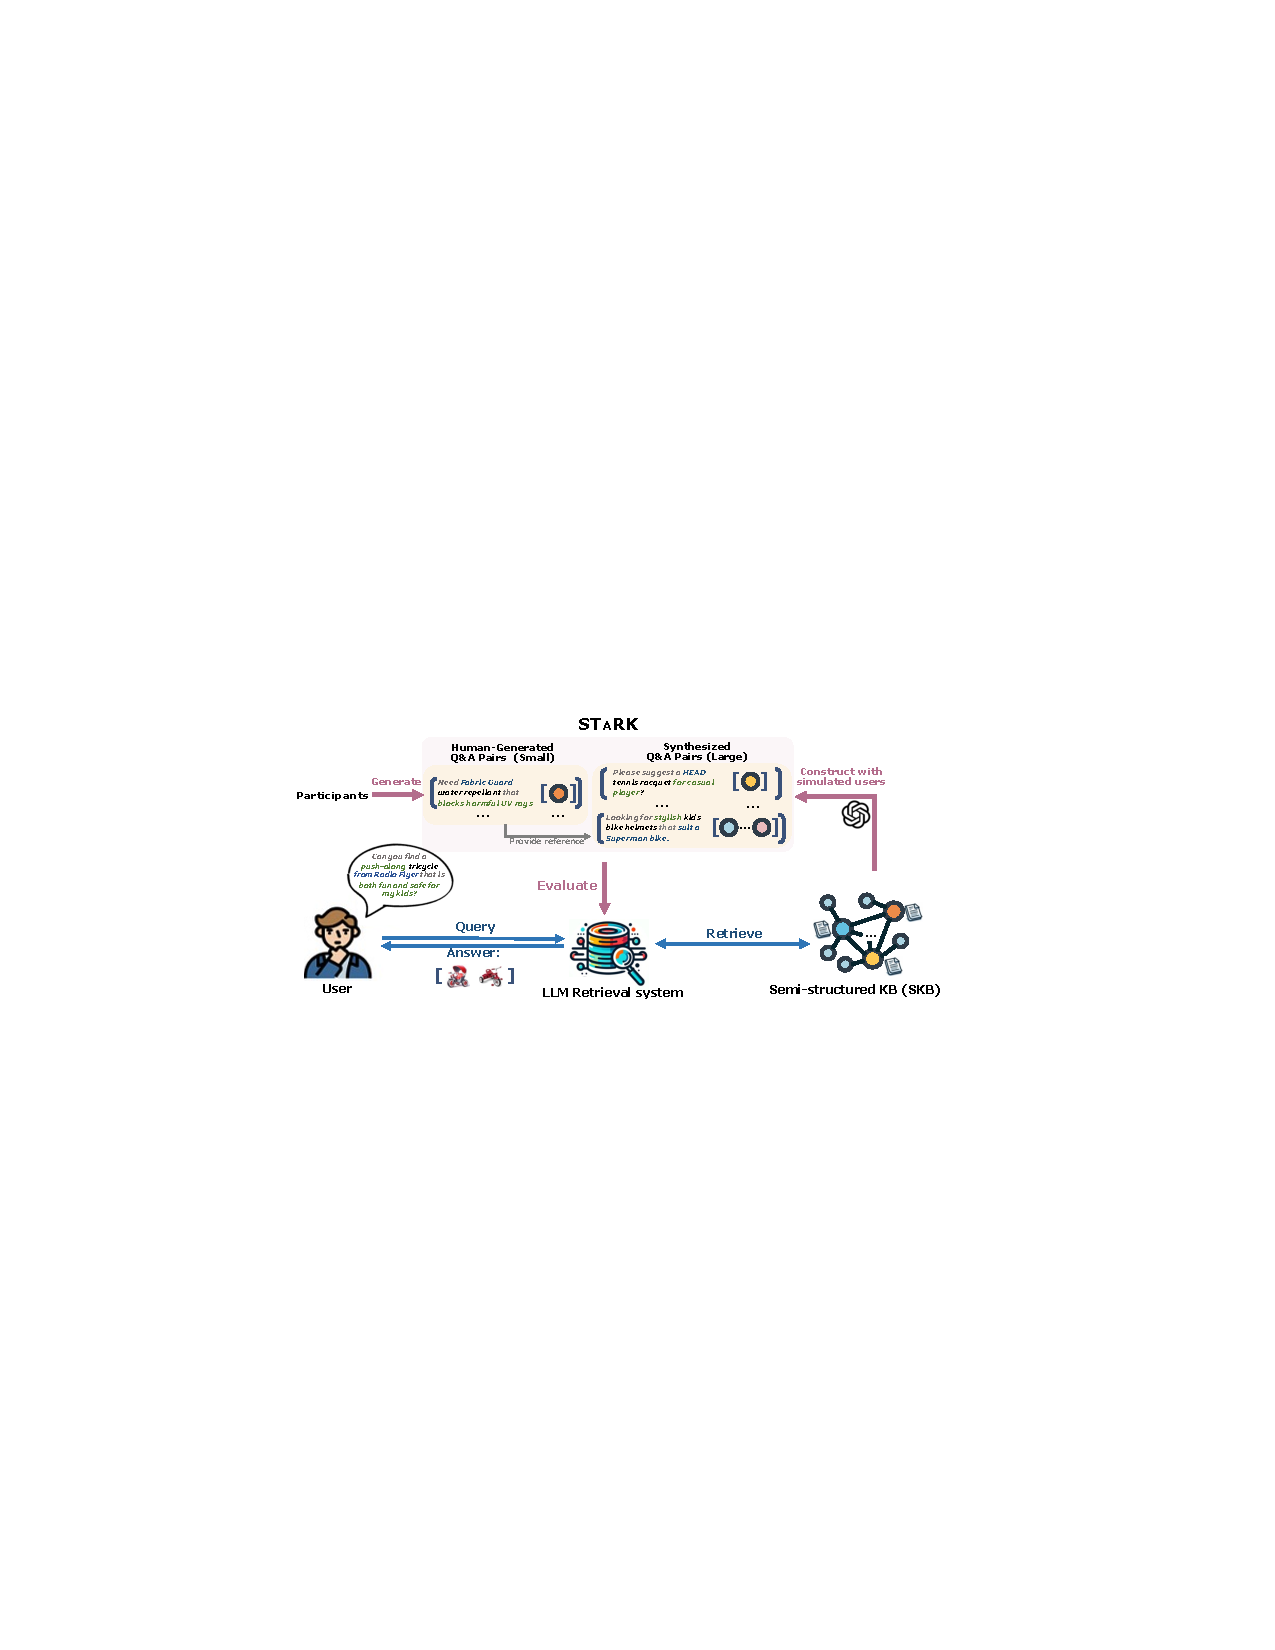
\includegraphics[width=0.90\textwidth]{figs/overview2}
    \caption{
    % Overview of the task and benchmark: 
    % Benchmarking retrieval systems on semi-structure knowledge bases with textual and relational information. 
    % \michi{Please provide more detailed caption to explain this figure. Whether Figure 1 is easy to understand or not is crucial, really influences readers' impression of this paper.}\kexin{i feel like it is hard to know where to start reading this figure. maybe add more annotations? for example, the upper part of figure can be shaded box and annotate with STAR benchmark and bottom part is the use case.}
    \benchmarkh features queries on Semi-structured Knowledge Base (SKB) with textual and relational knowledge, with node entities as ground-truth answers. \revision{\benchmarkh consists of synthesized queries simulating user interactions with a SKB and human-generated queries which provide an authentic reference. }It evaluates LLM retrieval systems' performance in providing accurate responses. 
    }
    \label{fig:task}
\end{figure}


% \begin{table}<t>
%     \resizebox{1.0\textwidth}{!}{
%     \begin{tabular}{ccc}
%         \toprule
%         & {Target} & {Example query} \\
%         \midrule
%         \hline
%         \multirow{4}{*}{\amazont} & \multirow{ 4}{*}{\texttt{product}} & \cellcolor{cyan!5} {\textit{Looking for \textcolor{OliveGreen}{durable} \textcolor{MidnightBlue}{Dart World brand} {dart flights} that}}\\
%          & & \cellcolor{cyan!5} {\textit{\textcolor{OliveGreen}{resist easy tearing}. Any recommendations?}}  \\
%         % \cellcolor{cyan!5} {\textit{Can you help me find a \textcolor{OliveGreen}{push-along} tricycle \textcolor{MidnightBlue}{from Radio Flyer} that's  }}  \\
%         % & & \cellcolor{cyan!5} {\textit{\textcolor{OliveGreen}{both fun and safe for my kid}?}}  \\
%         \noalign{\vspace{0.75ex}}
%         &&\cellcolor{cyan!5} {\textit{What are recommended {scuba diving weights} \textcolor{OliveGreen}{for experienced divers} }}\\
%         &&\cellcolor{cyan!5} {\textit{that would \textcolor{MidnightBlue}{fit well with my Gorilla PRO XL waterproof bag}?}}\\
%         \noalign{\vspace{0.7ex}}
%         \midrule
%         \noalign{\vspace{0.7ex}}
%         \multirow{ 3}{*}{\magt} & \multirow{ 3}{*}{\texttt{paper}} & \cellcolor{yellow!10} {\textit{Search {publications} \textcolor{MidnightBlue}{by Hao-Sheng Zeng} on \textcolor{OliveGreen}{non-Markovian dynamics}.}} \\
%         \noalign{\vspace{0.75ex}}
%         & &  \cellcolor{yellow!10}\textit{What are some \textcolor{OliveGreen}{nanofluid heat transfer} {research papers} published by}\\
%         & &  \cellcolor{yellow!10}\textit{scholars \textcolor{MidnightBlue}{from Philadelphia University}?} \cellcolor{yellow!10}\\
%         \noalign{\vspace{0.7ex}}
%         \midrule
%         \noalign{\vspace{0.75ex}}
%         \multirow{6}{*}{\primekgt} & \multirow{ 2}{*}{\texttt{drug}} &  \cellcolor{pink!20}\textit{Could you provide a list of \textcolor{OliveGreen}{investigational} {drugs} that }\\
%         && \cellcolor{pink!20}\textit{\textcolor{MidnightBlue}{interact with genes or proteins active in the epididymal region}?}\\
%         \noalign{\vspace{0.7ex}}
%         % & \multirow{ 1}{*}{\texttt{disease}}
%         % & \cellcolor{pink!20}\textit{Is my \textcolor{OliveGreen}{constant fatigue} due to conditions \textcolor{MidnightBlue}{related to bartonellosis}?}\\
%         & \multirow{ 2}{*}{\texttt{disease}}
%         & \cellcolor{pink!20}\textit{Search for {diseases} \textcolor{MidnightBlue}{without known treatments} and induce}\\
%         && \cellcolor{pink!20}\textit{\textcolor{OliveGreen}{pruritus in pregnant women}, potentially \textcolor{MidnightBlue}{associated with Autoimmune}.}\\
%         \noalign{\vspace{0.75ex}}
%         & \texttt{pathway} & \cellcolor{pink!20}\textit{Please find {pathways} \textcolor{MidnightBlue}{involving the POLR3D gene} \textcolor{OliveGreen}{within nucleoplasm}.}\\
%         \noalign{\vspace{0.75ex}}
%         & \texttt{gene} & \cellcolor{pink!20}\textit{Which {gene} on \textcolor{OliveGreen}{chromosome 4} are \textcolor{MidnightBlue}{expressed in multicellular organisms}?}\\
%         \bottomrule
%     \end{tabular}
%     }
%     \vspace{2pt}
%     \caption{Example queries from \benchmarkt, where \textcolor{MidnightBlue}{relational} and \textcolor{OliveGreen}{textual} aspects are highlighted.}
%     \label{tab:benchmark_examples}
%     \vspace{-10pt}
% \end{table}


% \begin{table}<t>
%     \resizebox{1.0\textwidth}{!}{
%     \begin{tabular}{lcl}
%         \toprule
%         &{Example query} & {Answer(s):}  \texttt{node\_id}$_{<\texttt{name/title}>}$\\
%         \midrule
%         \hline
%         \multirow{4}{*}{\small \amazont}& \cellcolor{cyan!5} {\textit{Looking for \textcolor{OliveGreen}{durable} \textcolor{MidnightBlue}{Dart World brand} {dart flights} that}} & \cellcolor{cyan!5} {\texttt{1082} {\tiny{<Amazon Standard Flights>}}} \\
%          & \cellcolor{cyan!5} {\textit{\textcolor{OliveGreen}{resist easy tearing}. Any recommendations?}}  & \cellcolor{cyan!5} {{\texttt{236112}} {\tiny{<Dart World Broken Glass Flight> (12 more)}}}  \\
%         \noalign{\vspace{0.75ex}}
%         &\cellcolor{cyan!5} {\textit{What are recommended {scuba diving weights} \textcolor{OliveGreen}{for experienced divers} }} & \cellcolor{cyan!5} {\texttt{1725} {\tiny{<Sea Pearls Vinyl Coated Lace Thru Weight>}}}\\
%         &\cellcolor{cyan!5} {\textit{that would \textcolor{MidnightBlue}{fit well with my Gorilla PRO XL waterproof bag}?}}& \cellcolor{cyan!5} {}\\
%         \midrule
%         \multirow{ 4}{*}{\small \magt}  & \cellcolor{yellow!10} {\textit{Search {publications} \textcolor{MidnightBlue}{by Hao-Sheng Zeng} on \textcolor{OliveGreen}{non-Markovian dynamics}.}} & \cellcolor{yellow!10} {{\texttt{1565109}} {\tiny{<Distribution of non-Markovian intervals...>}}} \\
%         &\cellcolor{yellow!10}{} &\cellcolor{yellow!10} {{\texttt{1628038}} {\tiny{<Comparison between non-Markovian...>}}}\\
%         \noalign{\vspace{0.75ex}}
%         & \cellcolor{yellow!10}\textit{What are some \textcolor{OliveGreen}{nanofluid heat transfer} {research papers} published by} & \cellcolor{yellow!10} {\texttt{1564849} {\tiny{<A Numerical Study on Convection}}}\\
%         &  \cellcolor{yellow!10}\textit{scholars \textcolor{MidnightBlue}{from Philadelphia University}?}  & \cellcolor{yellow!10} {{\tiny{Around A Suqare Cylinder using AL2O3-H2O Nanofluid>}}}\\
%         \midrule
%         \multirow{6}{*}{\small  \primekgt} &  \cellcolor{pink!20}\textit{Could you provide a list of \textcolor{OliveGreen}{investigational} {drugs} that } & \cellcolor{pink!20}\texttt{19756} {\tiny{<(S)-3-phenyllactic Acid>}}\\
%         &\cellcolor{pink!20}\textit{\textcolor{MidnightBlue}{interact with genes or proteins active in the epididymal region}?} & \cellcolor{pink!20}\texttt{19882} {\tiny{<Anisomycin>}}, \texttt{19883} {\tiny{<Puromycin>}}\\
%         \noalign{\vspace{0.75ex}}
%         % & \multirow{ 1}{*}{\texttt{disease}}
%         % & \cellcolor{pink!20}\textit{Is my \textcolor{OliveGreen}{constant fatigue} due nto conditions \textcolor{MidnightBlue}{related to bartonellosis}?}\\
%         & \cellcolor{pink!20}\textit{Search for {diseases} \textcolor{MidnightBlue}{without known treatments} and induce} & \cellcolor{pink!20}\texttt{27746} {\tiny{<Intrahepatic Cholestasis>}}\\
%         &\cellcolor{pink!20}\textit{\textcolor{OliveGreen}{pruritus in pregnant women}, potentially \textcolor{MidnightBlue}{associated with Autoimmune}.} & \cellcolor{pink!20}\\
%         \noalign{\vspace{0.75ex}}
%         & \cellcolor{pink!20}\textit{Please find {pathways} \textcolor{MidnightBlue}{involving the POLR3D gene} \textcolor{OliveGreen}{within nucleoplasm}.}& \cellcolor{pink!20}{\small{\texttt{128961}}}{\tiny{<RNA Polymerase III Chain Elongation> (4 more)}} \\
%         \noalign{\vspace{0.75ex}}
%         & \cellcolor{pink!20}\textit{Which {gene} on \textcolor{OliveGreen}{chromosome 4} are \textcolor{MidnightBlue}{expressed in multicellular organisms}?} & \texttt{1151} {\tiny{<NFKB1>}}, \texttt{13501} {\tiny{<MT2P1>}}\cellcolor{pink!20}\\
%         \bottomrule
%     \end{tabular}
%     }
%     \vspace{2pt}
%     \caption{Example queries from \benchmarkt, where \textcolor{MidnightBlue}{relational} and \textcolor{OliveGreen}{textual} aspects are highlighted.}\small{
%     \label{tab:benchmark_examples}
%     \vspace{-10pt}
% \end{table}


\begin{table}
    \resizebox{1.00\textwidth}{!}{
    \begin{tabular}{lcl}
        \toprule
        &{Example query} & Title of ground-truth items(s) \\
        \midrule
        \hline
        \multirow{4}{*}{\amazont}& \cellcolor{cyan!5} {\textit{Looking for \textcolor{OliveGreen}{durable} \textcolor{MidnightBlue}{Dart World brand} {dart flights} that}} & \cellcolor{cyan!5}  {\small{<Amazon Standard Flights>}} \\
         & \cellcolor{cyan!5} {\textit{\textcolor{OliveGreen}{resist easy tearing}. Any recommendations?}}  & \cellcolor{cyan!5} {{\small{<Dart World Broken Glass Flight> (+12 more)}}}  \\
        \noalign{\vspace{0.75ex}}
        &\cellcolor{cyan!5} {\textit{What are recommended {scuba diving weights} \textcolor{OliveGreen}{for experienced divers} }} & \cellcolor{cyan!5} {{\small{<Sea Pearls Vinyl Coated Lace Thru Weight>}}}\\
        &\cellcolor{cyan!5} {\textit{that would \textcolor{MidnightBlue}{fit well with my Gorilla PRO XL waterproof bag}?}}& \cellcolor{cyan!5} {}\\
        \midrule
        \multirow{ 4}{*}{\magt}  & \cellcolor{yellow!10} {\textit{Search {publications} \textcolor{MidnightBlue}{by Hao-Sheng Zeng} on \textcolor{OliveGreen}{non-Markovian dynamics}.}} & \cellcolor{yellow!10} {{\small{<Distribution of non-Markovian intervals...>}}} \\
        &\cellcolor{yellow!10}{} &\cellcolor{yellow!10} {{\small{<Comparison between non-Markovian...>}}}\\
        \noalign{\vspace{0.75ex}}
        & \cellcolor{yellow!10}\textit{What are some \textcolor{OliveGreen}{nanofluid heat transfer} {research papers} published by} & \cellcolor{yellow!10} {{\small{<A Numerical Study on Convection Around A}}}\\
        &  \cellcolor{yellow!10}\textit{scholars \textcolor{MidnightBlue}{from Philadelphia University}?}  & \cellcolor{yellow!10} {{\small{Suqare Cylinder using AL2O3-H2O Nanofluid>}}}\\
        \midrule
        \multirow{6}{*}{\primekgt} &  \cellcolor{pink!20}\textit{Could you provide a list of \textcolor{OliveGreen}{investigational} {drugs} that } & \cellcolor{pink!20}{ \small{<(S)-3-phenyllactic Acid>}},\\
        &\cellcolor{pink!20}\textit{\textcolor{MidnightBlue}{interact with genes or proteins active in the epididymal region}?} & \cellcolor{pink!20}{ \small{<Anisomycin>}}, {\small{<Puromycin>}}\\
        \noalign{\vspace{0.75ex}}
        & \cellcolor{pink!20}\textit{Search for {diseases} \textcolor{MidnightBlue}{without known treatments} and induce} & \cellcolor{pink!20} {\small{<Intrahepatic Cholestasis>}}\\
        &\cellcolor{pink!20}\textit{\textcolor{OliveGreen}{pruritus in pregnant women}, potentially \textcolor{MidnightBlue}{associated with Autoimmune}.} & \cellcolor{pink!20}\\
        \noalign{\vspace{0.75ex}}
        & \cellcolor{pink!20}\textit{Please find {pathways} \textcolor{MidnightBlue}{involving the POLR3D gene} \textcolor{OliveGreen}{within nucleoplasm}.}& \cellcolor{pink!20}{\small{<RNA Polymerase III Chain Elongation>}} \\ %  (4 more)
        \noalign{\vspace{0.75ex}}
        & \cellcolor{pink!20}\textit{Which gene or protein \textcolor{MidnightBlue}{associated with lichen amyloidosis} can }& {\small{<OSMR>}},  {\small{<IL31RA>}}\cellcolor{pink!20}\\
        & \cellcolor{pink!20}\textit{\textcolor{OliveGreen}{bind interleukin-31 to activate the PI3K/AKT and MAPK pathways}?}& \cellcolor{pink!20}\\
        %& \cellcolor{pink!20}\textit{Which {gene} on \textcolor{OliveGreen}{chromosome 4} are \textcolor{MidnightBlue}{expressed in multicellular organisms}?} & {\small{<NFKB1>}},  {\small{<MT2P1>}}\cellcolor{pink!20}\\
        \bottomrule
    \end{tabular}
    }
    \vspace{2pt}
    \caption{\benchmarkh QA examples which involve semi-structured (\textcolor{MidnightBlue}{relational} and \textcolor{OliveGreen}{textual}) information. }
    \label{tab:benchmark_examples}
    \vspace{-15pt}
\end{table}

\section{Introduction}
\vspace{-6pt}
%%%%% INTRODUCE THE PROBLEM SETTING %%%%%
Natural-language queries are the primary form of how humans acquire information~\cite{hirschman2001natural, kaufmann2010evaluating,Jamil17}. 
% landscape of 
% \kexin{what is diverse landscape of knowledge? are you referring to diverse domains?}
For example, users on e-commerce sites wish to express complex information needs by combining free-form elements and constraints, such as ``\textit{Can you help me find a push-along tricycle from Radio Flyer that’s both fun and safe for my kid?}''\revision{ in product search. Medical scientists may ask questions like ``\textit{What disease is associated with the PNPLA8 gene and presents with hypotonia as a symptom?}''}.
% \jure{Add one more example from some other domain: science or medical}
Answering such queries is crucial for enhancing user experience, supporting informed decision-making, and preventing hallucination.

To answer such queries, the underlying knowledge can be represented in %semi-structured formats~\cite{UniK-QA,mag,RyuJK14}, referred to as 
semi-structured knowledge bases (SKBs)~\cite{UniK-QA,mag,RyuJK14}, which integrate unstructured data, such as natural language descriptions and expressions (\eg description of the tricycle), with structured data, like entity interactions on knowledge graphs
%\qian{I think using database is better, maybe database graph?} 
(\eg a tricycle ``brand'' is Radio Flyer). 
This allows the SKBs to represent comprehensive knowledge in specific applications, making them indispensable in domains such as e-commerce~\cite{ups-amazon_review}, social media~\cite{MansmannRWS14}, and precision medicine~\cite{primekg, ogb, Johnson2021}.

%%%% THE PROBLEM WE WANT TO SOLVE %%%%%%
%%%% + Why IS THIS IMPORTANT %%%%%%
%In this context, as shown in Figure~\ref{fig:task}, information retrieval serves as a predominant step by identifying relevant data from the SKBs, such as specific tricycles that match the request, which are then processed to generate accurate answers to user queries~\cite{Singhal01}.
%The retrieval accuracy on SKBs is crucial for enhancing user experience, supporting informed decision-making, and preventing hallucination.

%%%%%%%%%%% WHY HASN'T IT BEEN SOLVED %%%%%%%%
\xhdr{Limitations of prior works} Prior works focused on either purely textual queries on unstructured knowledge~\cite{IzacardG21, realm, KarpukhinOMLWEC20, LeeCT19, YangXLLTXLL19, dunn2017searchqa, TriviaQA, yang2018hotpotqa} or structured SQL~\cite{zhongSeq2SQL2017, yu-etal-2018-spider, zhongSeq2SQL2017, yu-etal-2018-spider} or knowledge graph queries~\cite{BerantCFL13, YihCHG15, h2t, ComplexWebQuestions, yih-etal-2016-value,talmor-berant-2018-web,cao-etal-2022-kqa,GAO_FODOR_KIFER_2019,he2024gretriever,AsaiHHSX20}, which are limited in the span of knowledge and inadequate to study the complexities of retrieval on SKBs. Recently, large language models (LLMs) have demonstrated significant potential on information retrieval tasks~\cite{llm4ir, realm, rag, replug}. Nevertheless, it remains an open question of how effectively LLMs can be applied to the challenging retrieval tasks on SKBs.  Moreover, the existing works mainly focus mainly on general knowledge, \eg from Wikipedia. However, the knowledge may commonly come from private sources, requiring retrieval systems to \revision{operate} on private SKBs. Therefore, there is a gap of how current LLM retrieval systems handle the complex textual and relational requirements in queries that can involve private knowledge. 

%%%%%%%%% WHY IS IT HARD %%%%%%%%%
% \kexin{i feel like here misses a transition sentence. Before here, you are discussing about this new problem setting of SKB and how previous works do not address them. In the next paragraph, you jump into talking about de details of building a benchmark for it. But you haven't motivated why do we need a benchmark for it and why is it hard to build this benchmark. }
\xhdr{Present work} 
To address this gap, we present a large-scale \underline{S}emi-structure retrieval benchmark on \underline{T}extual \underline{a}nd \underline{R}elational \underline{K}nowledge Bases (\benchmarkt) (Figure~\ref{fig:task}). The key technical challenge that we solve is how to accurately simulate user queries on SKBs. This difficulty arises from the interdependence of textual and relational information, which leads to challenges in precisely construct the ground-truth answers from millions of candidates. Additionally, ensuring that queries are useful and resembles real-world scenarios adds further complexity to the benchmarking process. 
 
We develop a novel pipeline that simulates user queries and constructs precise ground truth answers using three SKBs built from extensive texts and millions of entity relations from public sources.
We validate the quality of queries in our benchmark through detailed analysis and human evaluation, focusing on their naturalness, diversity, and practicality.
\revision{Furthermore, we incorporate 274 human-generated queries to compare with synthesized queries and enrich the testing scenarios.} With \benchmarkt, we delve deeper into retrieval tasks on SKBs, evaluate the capability of current retrieval systems, and provide insights for future advancement. 
Key features of \benchmarkh are:
\begin{itemize}[leftmargin=*]
    \vspace{-5pt}
    % \item \textbf{Semi-structured and \qian{the query is just unstructured natural language right? } natural-sounding queries:} 
    \item \textbf{Natural-sounding queries on SKBs (Table~\ref{tab:benchmark_examples}):} Queries in our benchmark incorporate rich relational information and complex textual properties. Additionally, these queries closely mirror the types of questions users would naturally ask in real-life scenarios, \eg with flexible query formats and possibly with additional contexts.
    \vspace{-1pt}
    \item \textbf{Context-specific reasoning:} The queries entail reasoning capabilities specific to the context. This includes the ability to infer customer interests, understand specialized field descriptions, and deduce relationships involving multiple subjects mentioned within the query.
    % \qian{Not sure I understand this feature. Do you mean query-specific? what is the context?}
    For example, the context  ``\textit{I had a dozen 2.5-inch Brybelly air hockey pucks, so I'm trying to find matching strikers.}'' entails the user's interest in looking for complementary products.
    Such reasoning capabilities are crucial for accurately interpreting and responding to the nuanced requirements of each query. 
    \vspace{-1pt}
    \item \textbf{Diverse domains:} 
    Our benchmark spans three knowledge bases\footnote{Explore the SKBs at \textcolor{cyan}{\url{https://stark.stanford.edu/skb_explorer.html}}} for applications including product recommendation, academic paper search, and precision medicine inquiries. \benchmarkh provides a comprehensive evaluation of retrieval systems across diverse contexts and domains. 
\end{itemize}

\vspace{-5pt}
We conduct extensive experiments on LLM retrieval systems, highlighting challenges in handling textual and relational data and latency on large-scale SKBs with millions of entities or relations. Finally, we offer insights into building more capable retrieval systems to handle real-world complexity.



% In the realm of information retrieval, semistructured queries have emerged as a natural and intuitive means of expressing complex information needs. Such queries allow users to combine free-form textual elements with structured constraints, enabling more precise and nuanced searches. However, despite their potential, the development of benchmarks to evaluate the effectiveness of retrieval systems in handling semistructured queries has been limited.

% However, few have been developed for complex retrieval tasks.\\
% Previous works have focused on either textual or SQL queries\\
% Previous works simplify problems \\
% The primary challenge lies in the complexity of these retrieval tasks. Previous works have predominantly focused on either purely textual queries or strictly structured SQL queries, often simplifying the problem to fit within these paradigms. As a result, there is a gap in our understanding of how well current systems can handle the intricate interplay between textual and relational information present in semistructured queries.


% We design a novel pipeline to build the benchmark\\
% To address this gap, we propose a novel benchmarking pipeline specifically designed for semistructured information retrieval. Our benchmark, \benchmarkt, is a large-scale dataset that requires systems to leverage both textual and relational knowledge. It is crafted to resemble real-world settings and spans diverse domains, providing a comprehensive testbed for evaluating retrieval systems.


%%%%%%%%% HOW WELL DOES IT PERFORM %%%%%%%%%%%
% It exhibits explicit and rich relational information from (private) KB, complex textual properties, natural-sounding queries. Table~\ref{tab:benchmark_examples}
% Our benchmark stands out in its ability to present explicit and rich relational information from private knowledge bases, alongside complex textual properties and natural-sounding queries. This combination ensures that the evaluated systems must possess a deep understanding of both text and structure to succeed. Table~\ref{tab:benchmark_examples} provides examples from our benchmark, illustrating the variety and complexity of the queries.


\vspace{-5pt}
\section{Benchmarking 
Retrieval Tasks over Textual and Relational Knowledge}
\vspace{-5pt}
% We develop three large-scale retrieval datasets on three semi-structured knowledge bases (SKBs) In Section~\ref{sec:def}, we introduce SKB and the problem setting.
% In Section~\ref{sec:skb}, we introduce the schema and scale of the SKBs, which integrate entities with rich relational and textual information. 
% In Section~\ref{sec:star}, we introduce the retrieval datasets and the key characteristics of the queries. Then, we highlight our novel dataset construction pipeline in Section~\ref{sec:construction}, which simulates user queries involving textual and relational knowledge and automatically generates the ground truth answers in the retrieval datasets.
% Finally, we conduct data distribution analysis and human evaluation on the queries in Section~\ref{sec:analysis}.
% % These knowledge bases integrate entities with detailed relational and textual information. 
% % Then the retrieval datasets are constructed in a way that assesses the model's proficiency in extracting information from varied data structures and synthesizing it to generate correct answers.

% \jure{You can cut this summary paragraph with forward references. It is a waste fo space}
% \jure{Instead you can have a section where you formally define the problem: We consider the following setting: SOMETHING LIKE THIS (PLEASE POLISH): We are given SKB, which is composed of a Knowledge Graph $G$ with a set of nodes and relations. We also assume that with each node $i$ there is a set of associated free text documents $D_i$. For example, in e-commerce, Knowledge Graph is a product knowledge graph capturing properties of products (brand, color) and the text documents correspond to reviews and product descriptions. Now given a Query $Q$, our goal is to find a set of answers that match the query. Answers are a subset of items in the knowledge graph. For example, in e-commerce answers are actual products.}


\begin{figure}[t]
    \centering
    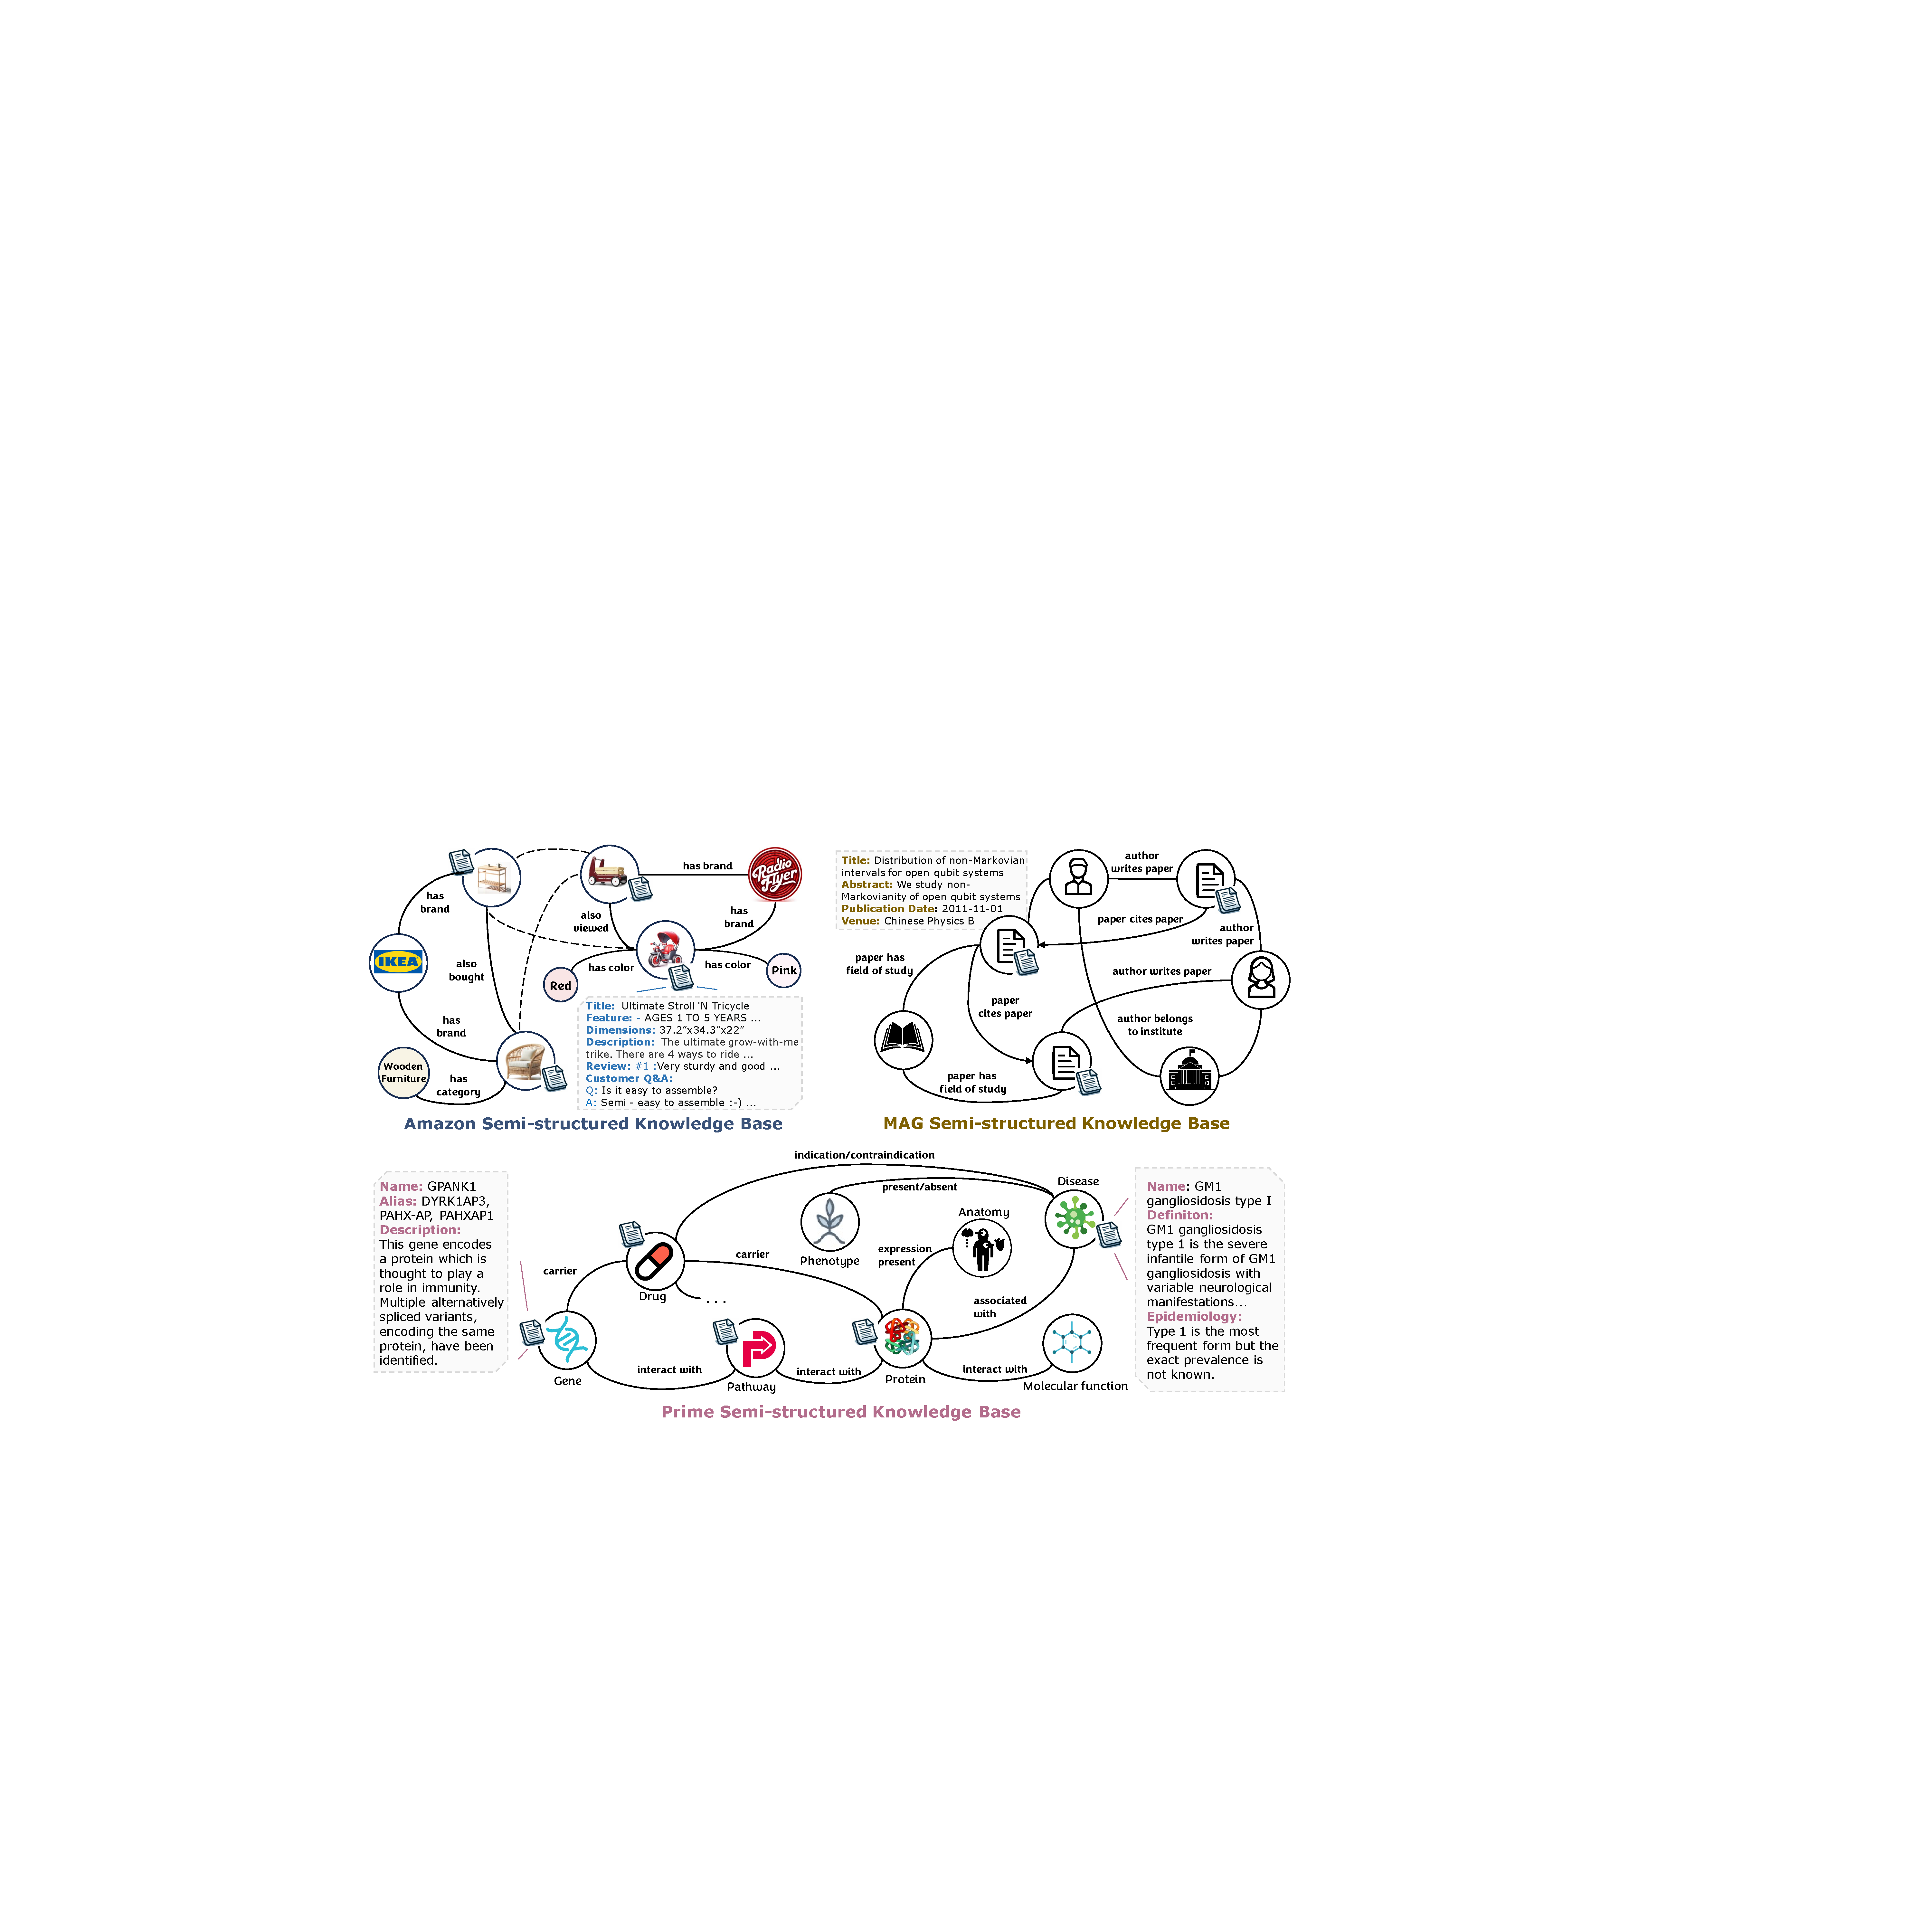
\includegraphics[width=0.98\textwidth]{figs/semistructure_v2}
    \vspace{-5pt}
    \caption{Demonstration of Semi-structured Knowledge Bases, 
    %\michi{You can also mention what you want readers to take away from this, e.g. "observe that semi-structured KB consists of text and relational info, which makes the task hard", etc.}
    where each knowledge base combines both textual and relational information in a complex way, making the retrieval tasks challenging.
    }
    \vspace{-15pt}
    \label{fig:semistructure}
\end{figure}

\subsection{\revision{Problem Definition}}
\label{sec:def}
\vspace{-3pt}
We are given a Semi-Structured Knowledge Base (SKB), which consists of a knowledge graph \( G \) and a collection of free text documents  $D$. 
% The knowledge graph \( G = (V, E) \) is composed of a set of nodes \( V \) and a set of edges \( E \), where each edge represents a relational link between nodes. Each node \( i \in V \) has an associated set of free text documents \( D_i \). 
Formally, let \( G = (V, E) \) be the knowledge graph, where \( V \) is the set of nodes and \( E \subseteq V \times V \) is the set of edges representing relationships between nodes. \( D = \bigcup_{i \in V} D_i \) be the collection of free-form text documents associated with the nodes, where \( D_i \) is the set of documents associated with node \( i \). For example, the product knowledge graph in e-commerce can capture relationships between products and brands/colors/categories, and the corresponding text documents include product descriptions, reviews, \etc

We define the tasks on our benchmark datasets as follows: 
Given the knowledge graph \( G = (V, E) \), a collection of free text documents \( D \), and a query \( Q \), the output is a set of nodes \( A \subseteq V \) such that for each node \( i \in A \), it satisfies the relational requirements imposed by the structure of \( G \) as specified in \( Q \), and the associated documents \( D_i \) satisfy the textual requirements specified in \( Q \). 

% v2: This work addresses semi-structured knowledge base retrieval, integrating relational and textual data extraction from databases \( \mathcal{D} = \{R, T\} \), with \( R \) and \( T \) representing relational and textual data, respectively. The objective is to construct a model \( f \) that, given a query \( Q = \{Q_r, Q_t\} \), maps it to an answer \( A \). The answer \( A \) are nodes in \( \mathcal{D} \) satisfying both relational \( Q_r \) and textual \( Q_t \) query parts. The task is defined as finding \( f: \{Q_r, Q_t\} \times \mathcal{D} \rightarrow A \), effectively merging \( R \) and \( T \) to generate \( A \). The input of the model is semi-structure knowledge base and a query, and the output should be a set of predicted answers.

\vspace{-3pt}
\subsection{Semi-structured Knowledge Bases (SKBs)}
\label{sec:skb}
\vspace{-3pt}

\begin{table}[t]
    \centering
    \caption{Data statistics of our constructed semi-structured knowledge bases}
    \resizebox{0.92\textwidth}{!}{
    \begin{tabular}{l|ccrrrr}
        \toprule
        \multirow{ 2}{*}{} & \textbf{\#entity} & \textbf{\#relation} & \textbf{avg. } & \multirow{ 2}{*}{\textbf{\#entities}} & \multirow{ 2}{*}{\textbf{\#relations}} & \multirow{ 2}{*}{\textbf{\#tokens}} \\
        & \textbf{types} &\textbf{types} & \textbf{degree}\\
        \midrule
        \amazont & 4 & 5  & 18.2 & 1,035,542 & 9,443,802 & 592,067,882\\
        \magt & 4 & 4  & 43.5& 1,872,968 & 39,802,116 & 212,602,571\\
        \primekgt & 10& 18 & 125.2 & 129,375 & 8,100,498  & 31,844,769\\
        \bottomrule
    \end{tabular}
    }
    \vspace{-15pt}
    \label{tab:statistics}
\end{table}

As shown Figure~\ref{fig:semistructure}, we construct three large-scale SKBs with the relational and textual information with each entity. 
See Table~\ref{tab:statistics} for the basic data statistics and Appendix~\ref{app:skb} for details.
% \karthik{Refer this table at the end of this section along with other Appendices. Seems out of place.}
% See Table~\ref{tab:sources} for the comprehensive public sources we used to construct the SKBs. 

\xhdr{Amazon Semi-structured Knowledge Base}  
The SKB features four entity types: \texttt{product}, \texttt{brand}, \texttt{color}, and \texttt{category}, and five relation types:  \texttt{also\_bought, also\_viewed} between \texttt{product} entities, and
\texttt{has\_brand/color/category} associated with the products. 
We derive the textual information of \texttt{product} nodes by combining Amazon Product Reviews~\cite{ups-amazon_review} with Amazon Q\&A Data~\cite{image_amazon_qa}. 
This provides a rich amount of texts, including product descriptions and customer reviews. 
For other entities, we extract their names or titles as the textual attributes. Amazon SKB features an extensive textual data largely contributed from customer reviews and Q\&A.

\xhdr{MAG Semi-structured Knowledge Base} 
This SKB includes node entities of \texttt{paper}, \texttt{author}, \texttt{institute}, and \texttt{field\_of\_study}. We derive its relational structure by extracting a subgraph from obgn-mag~\cite{hu2021open}, which contains shared paper nodes with obgn-papers100M~\cite{hu2021open} and all non-paper nodes. We filter out non-English language papers as we only consider single-lingual queries. 
The paper documents include their titles and abstracts. Additionally, we integrating details from the Microsoft Academic Graph database (version 2019-03-22)~\cite{mag, mag_data}, providing extra textual information like paper venue, author and institution names. 
This SKB demonstrates a large number of relations associate with \texttt{paper} nodes, especially on citation and authorship relations. 


\xhdr{Prime Semi-structured Knowledge Base} We leverage the exisiting knowledge graph PrimeKG~\cite{primekg} which contains ten entity types including \texttt{disease, gene/protein}, and eighteen relation types, such as \texttt{associated\_with, indication}.
Compared to the Amazon and MAG SKBs, Prime SKB is denser and features a greater variety of relation types. While PrimeKG provides text information on \texttt{disease} and \texttt{drug} entities, 
% including drug mechanisms and disease descriptions, 
we integrate the data from multiple databases for \texttt{gene/protein} and \texttt{pathway} entities such as genomic position, gene activity summary and pathway orthologous event.





\subsection{Retrieval Tasks on Semi-structured Knowledge Bases}
\label{sec:star}
Our retrieval benchmark (Table~\ref{tab:benchmark_stats}) consists of three novel retrieval-based question-answering datasets, each comprising synthesized train/val/test sets with $9$k to $14$k queries in total and a high-quality human-generate query set.
% Specifically, the task is to retrieve items  over the SKBs given any input queries. 
The queries synthesize relational and textual knowledge, mirroring real-world queries in terms of natural-sounding property and flexible formats.

% Our retrieval benchmark, detailed in Table~\ref{tab:benchmark_stats}, comprises between $9$k to $14$k queries per dataset. Below, we outline the task on each dataset:

% Each query may have single answer or multiple answers, formulated as a subset of entities \revision{in the knowledge graph,}
% \jure{This is wrong. Entities are in the knowlede graph, Knowledge Base contains documents as well but those are not answers}
% which requires the model to accurately identify the ground truth entities out of potentially millions in response to each query.
% In Table~\ref{tab:benchmark_examples}, we demonstrate example queries from these benchmarks. 
\xhdr{\amazont} 
% This dataset comprises 9,100 synthesized customer-focused queries \hw{along with 81 human-generated queries for additional evaluation}. 
The task aims at product recommendation, with a notable 68\% of the synthesized queries yielding more than one ground truth answer. The dataset prioritizes customer-oriented criteria, highlighting textual elements such as product quality, functionality, and style. Moreover, it incorporate single-hop relational aspects (Appendix~\ref{app:amazon}) into the queries, including brand, category, and product connections (\eg complementary or substitute items). The queries are framed in conversation-like formats, enriching the context and enhancing the dataset's relevance to real-world scenarios.


% true positive: 86.6\%
% true negative: 96.7\%
\xhdr{\magt} 
% This dataset comprises 13,323 synthesized \hw{and 84 human-generated queries targeting at academic paper search.} 
Beyond the single-hop relational requirements in \amazont, \magh emphasizes the fusion between the textual requirements with multi-hop queries for precise academic paper search. For example, ``Are there any papers from King's College London'' highlights the metapath (\texttt{institution $\rightarrow$ author $\rightarrow$ paper}) on the relational structure. 
We designed three single-hop and four multi-hop relational query templates (Appendix~\ref{app:mag}). The textual aspects focus on the paper's topic, methodology, and contribution \etc
% true positive: 98.9\%

\xhdr{\primekgt} 
% This dataset, comprising 11,204 synthesized queries and \hw{109 human-generated queries across all ten entity types,} incorporates single-hop and multi-hop relational information similar to \magt. 
% For synthesized queries, we developed 28 multi-hop query templates, detailed in Appendix~\ref{app:prime}, to cover various relation types and ensure their practical relevance. 
% For instance, the query ``What is the drug that targets the genes or proteins expressed in <anatomy>?'' serves applications in precision medicine and pharmacogenomics, 
% aiding researchers and healthcare professionals in identifying drugs that act on genes or proteins associated with specific anatomical areas and enabling more targeted treatments. 
The task is to answer complex biomedicine inquiries. 
For synthesized queries, we developed 28 multi-hop query templates (Appendix~\ref{app:prime}) to cover various relation types and ensure their practical relevance. 
For example, the template ``What is the drug that targets genes or proteins in <anatomy>?'' aids precision medicine by identifying treatments targeted to specific anatomical areas.
For \texttt{drug, disease, gene/protein}, and \texttt{pathway} entities, the queries are a hybrid of relational and textual requirements. 
For entities such as \texttt{effect/phenotype}, the queries rely solely on relational data due to limited textual information. 
We exhibit three distinct user roles – medical scientist, doctor, and patient – for generating queries about drug and disease, which diversify the language to comprehensively evaluate the retrieval systems.



\begin{table}[t]
    \centering
    \caption{Statistics on the \benchmarkh benchmark datasets.}
    \resizebox{0.9\textwidth}{!}{
    \begin{tabular}{ll|rrrr}
        \toprule
        & & \multirow{2}{*}{\textbf{ \#queries}}  & \textbf{ \#queries w/} & \textbf{average} & \multirow{2}{*}{\textbf{train / val / test}}\\
        & & & \textbf{multiple answers}&  \textbf{\#answers} & \\
        \midrule
        \multirow{3}{*}{
        \makecell{Synthesized\\
        (Sec~\ref{sec:construction}, \ref{sec:analysis})}} & {\small \amazont} & 9,100 & 7,082  & 17.99& {0.65 / 0.17 / 0.18}\\
        & {\small \magt} &13,323 & 6,872 & 2.78 & {0.60 / 0.20 / 0.20}\\
        & {\small \primekgt} & 11,204 & 4,188 & 2.56 & {0.55 / 0.20 / 0.25} \\
        \midrule
        \multirow{3}{*}{\makecell{Human-generated\\
        (Sec~\ref{sec:human_generated})}} 
        & {\small \amazont} & 81 & 64 & 19.50 & \multirow{3}{*}{For testing only}\\
        & {\small \magt} & 84 &34 & 3.26 & \\
        & {\small \primekgt} & 98 & 41 & 2.77 & \\
        \bottomrule
        \end{tabular}
        }
    \vspace{-5pt}
    \label{tab:benchmark_stats}
\end{table}
\begin{figure}[t]
    \centering
    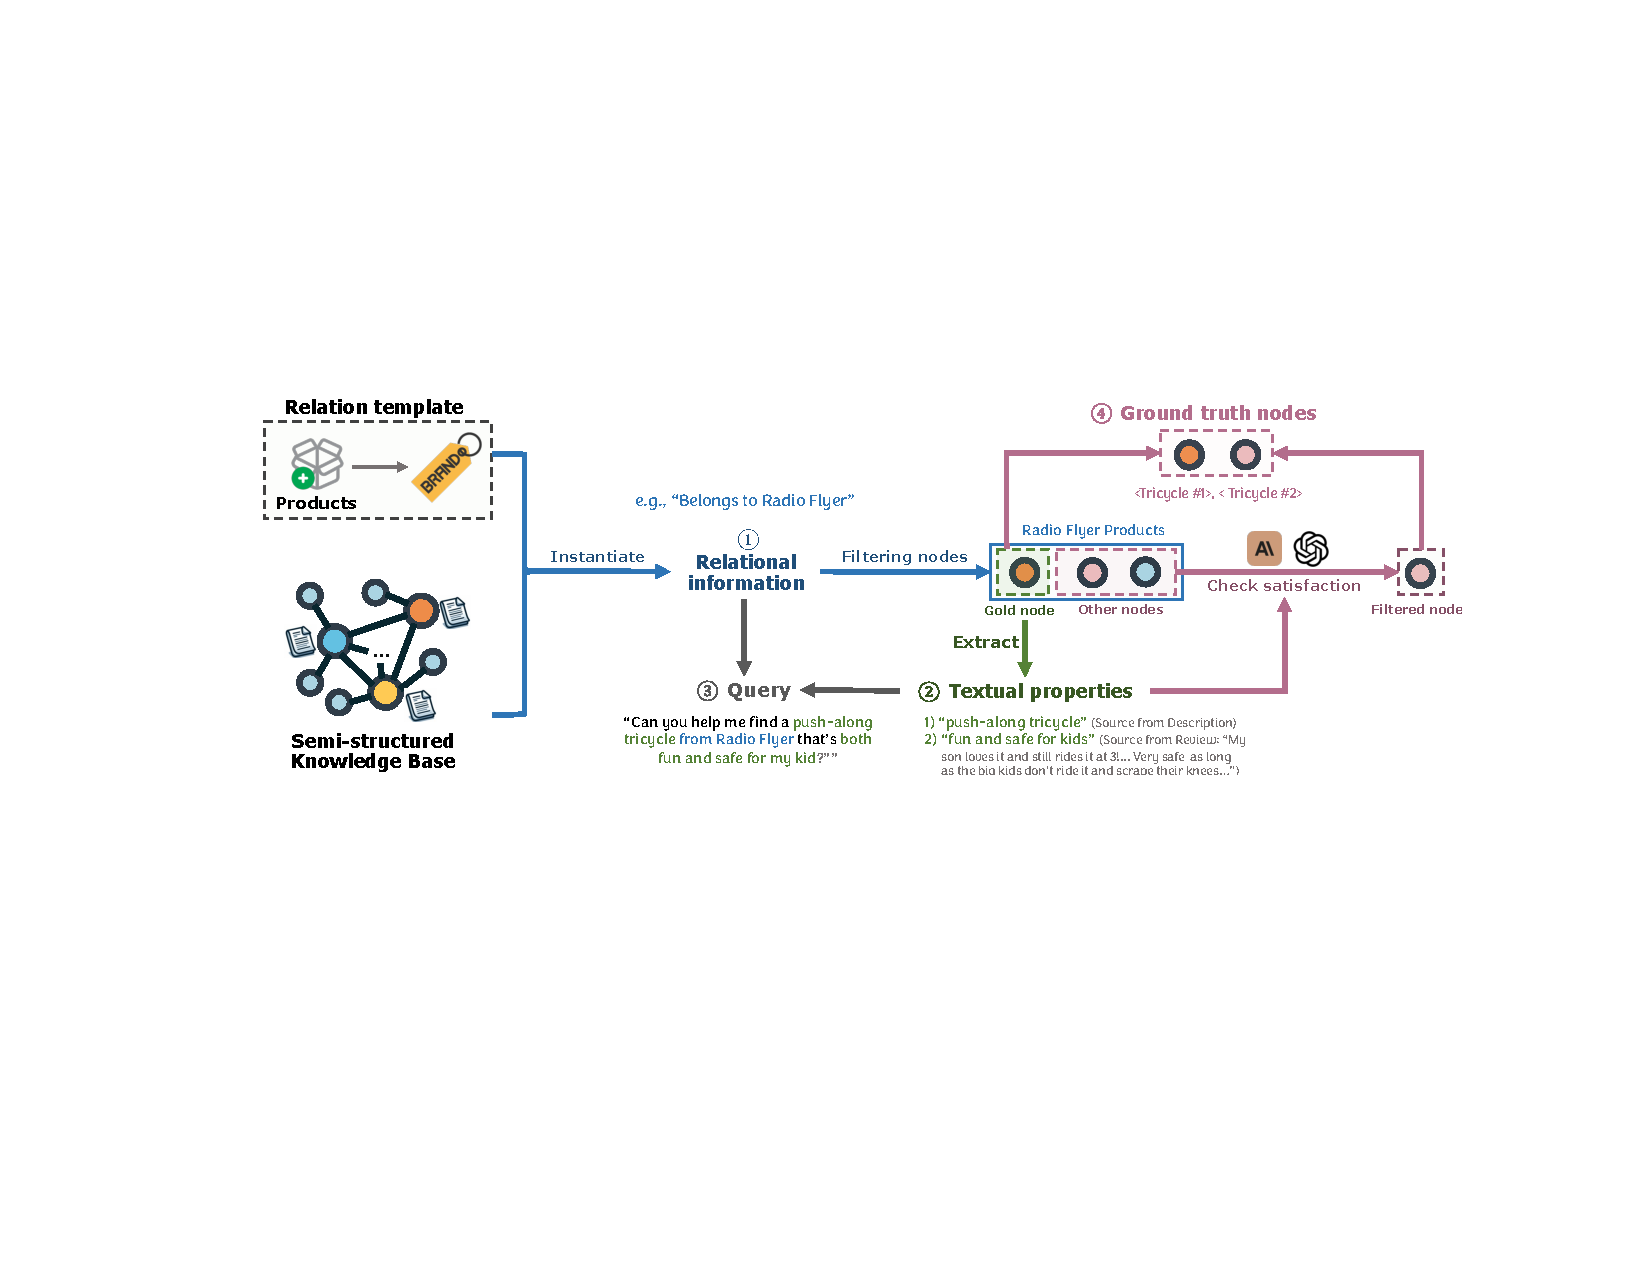
\includegraphics[width=0.95\textwidth]{figs/construction}
    \vspace{-3pt}
    \caption{
    The construct pipeline to generate our semi-structured retrieval datasets.
    % involves four main steps: 1) Sample Relational Requirement: Based on relational templates, sample a relational requirement on a SKB.
    % 2) Extract Textual Properties: From a node that meets the relational requirement, extract relevant textual properties.
    % 3) Combine Information: Merge the relational information and textual properties to form a natural-sounding query.
    % 4) Construct Ground Truth Nodes: Check if nodes satisfy the textual properties using multiple language models to establish ground truth nodes.
    }
    \vspace{-10pt}
    %\kexin{what is the meaning of edge color?}
    %\shirley{the edge colors are made the same as the arrow color}
    \label{fig:construction}
\end{figure}

\vspace{-2pt}
\subsection{Benchmark Construction: Synthesized Queries} 
\label{sec:construction}
\vspace{-2pt}
% \karthik{this section needs a running example and should be tied closely to the numbering in Fig 5}
In Figure~\ref{fig:construction}, we present a novel pipeline that synthesizes the SKB queries and automatically generates the ground truth answers. 
The key idea is to entangle relational and textual information during synthesis and disentangle them during answer filtering. 
It involves four steps as follows:
% The pipeline involves four steps and the specific processes vary depending on the characteristics of each dataset. These steps are as follows:

% We leverage the GPT and Claude language models to construct the retrieval datasets. Detailed descriptions of all the prompts we used are available in Appendix~\ref{app:prompts}. 

\begin{itemize}[leftmargin=*]
\vspace{-2pt}
\item \textbf{1) Sample Relational Requirements:} For each query, we sample a practical relation template constructed with expert/domain knowledge, \eg ``\texttt{(a product) belongs to <brand>}'' and ground it with sampled entities (\ie a specific brand), \eg ``belongs to Radio Flyer''. 
This relational requirement yields a set of candidate entities, \ie products belonging to Radio Flyer. 
% \revision{The relation templates for the three SKBs are practical and constructed with expert/domain knowledge}, which are available in Appendix~\ref{app:details}. 
% Therefore, we obtain the relational requirements and the corresponding candidates. 
% For instance, the template ``What is the drug that targets the genes or proteins which are expressed in <anatomy>?'' is particularly valuable for precision medicine inquiries. It aids in pinpointing medications aimed at specific genetic or protein targets within defined anatomical areas, thereby contributing to the development of targeted treatments. 
% \shirley{relate text to figure, \eg step 1}
\vspace{-2pt}
\item \textbf{2) Extracting Textual Properties:} \revision{
% The relational requirement yields a set of satisfying candidates. 
We randomly sample a candidate entity from the first step, referred to as the \textit{gold answer}, from which LLMs extract properties that align with the interests of specific roles (\eg customers, researchers, or doctors) in its textual document}.  In Figure~\ref{fig:construction}, we extract multiple properties about the functionality and user experience from a Radio Flyer product. 
%%%%%% We utilize GPT-3.5-turbo-16k for the \amazonh and Claude-v2 for the other two datasets to conduct this step, where the prompts used are included in Appendix~\ref{app:prompts}.  
% \karthik{how?}
\vspace{-2pt}
\item \textbf{3) Combining Textual and Relational Information:} 
We use two LLMs to synthesize queries from textual properties and relational requirements, enhancing diversity and reducing bias arise from relying on a single LLM. 
The first LLM focuses on generating natural, role-specific, and style-consistent (\eg ArXiv searches) queries. The second LLM enriches the context and rephrases queries, which poses the need for advanced reasoning to comprehend them under complex contexts.

\vspace{-2pt}
\item \textbf{4) Filtering Additional Answers:} 
Finally, we employ multiple LLMs to verify if the candidates from the first step meet the extracted textual properties. Only candidates passing all LLM verifications are included in the final ground truth set. To assess the precision of this filtering mechanism, we compute the average ratios for the gold answers to be verified, which are 86.6\%, 98.9\%, and 92.3\% on the three datasets, highlighting our efficacy in yielding high-quality ground truth answers.

\vspace{-2pt}
\end{itemize}

This dataset construction pipeline is automatic, efficient, and broadly applicable to the SKBs in our formulation.  
\revision{We include all of the prompts and the LLMs versions in the above steps in Appendix~\ref{app:prompts}.} 



\begin{figure}[t]
    \centering
    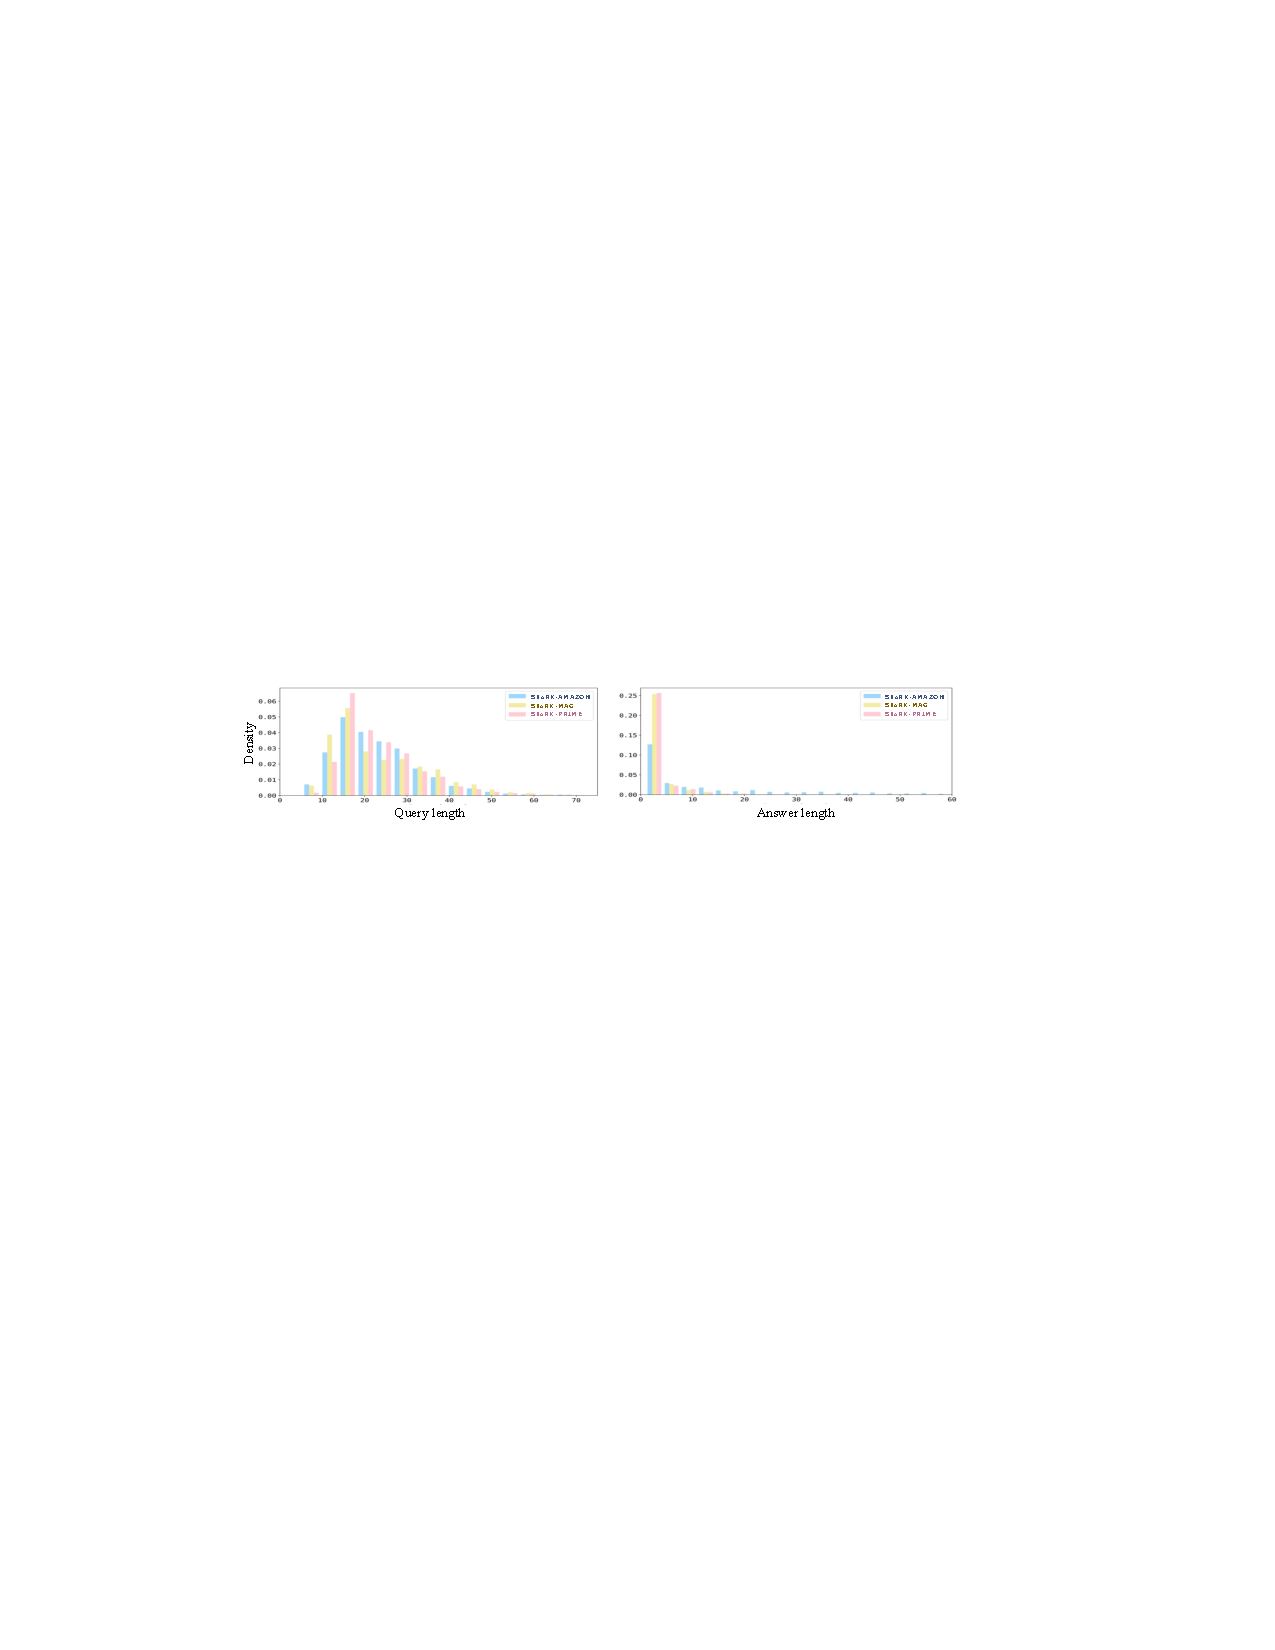
\includegraphics[width=1\textwidth]{figs/length_histv2}
    \vspace{-15pt}
    \caption{Distribution of query and answer lengths on \benchmarkh datasets.}
    \vspace{-5pt}
    \label{fig:length_dist}
\end{figure}

\begin{figure}[t]
    \begin{minipage}[t]{0.5\textwidth}
        \centering
      \captionof{table}{Query diversity measurement on \benchmarkt. \revision{See Appendix~\ref{app:math} for the metric definition.}}
      \vspace{5pt}
        \resizebox{1\textwidth}{!}{
        \begin{tabular}{l|cc}
            \toprule
            & {\small Shannon Entropy} & {\small Type-Token Ratio} \\
            % & {\small Entropy} & {\small Ratio} \\
            \midrule
            \small \amazonh & 10.39 & 0.179 \\
            \small \magh & 10.25 & 0.180 \\
            \small \primekgh & 9.63 & 0.143 \\
            \midrule
            \small Reference article & 10.44 & 0.261\\
            \bottomrule
        \end{tabular}
        }
        \label{tab:q_diversity}
    \end{minipage}%
    \hfill 
    \begin{minipage}[t]{0.47\textwidth}
        \caption{Average relative composition of relational vs. textual information.}
        \vspace{-5pt}
        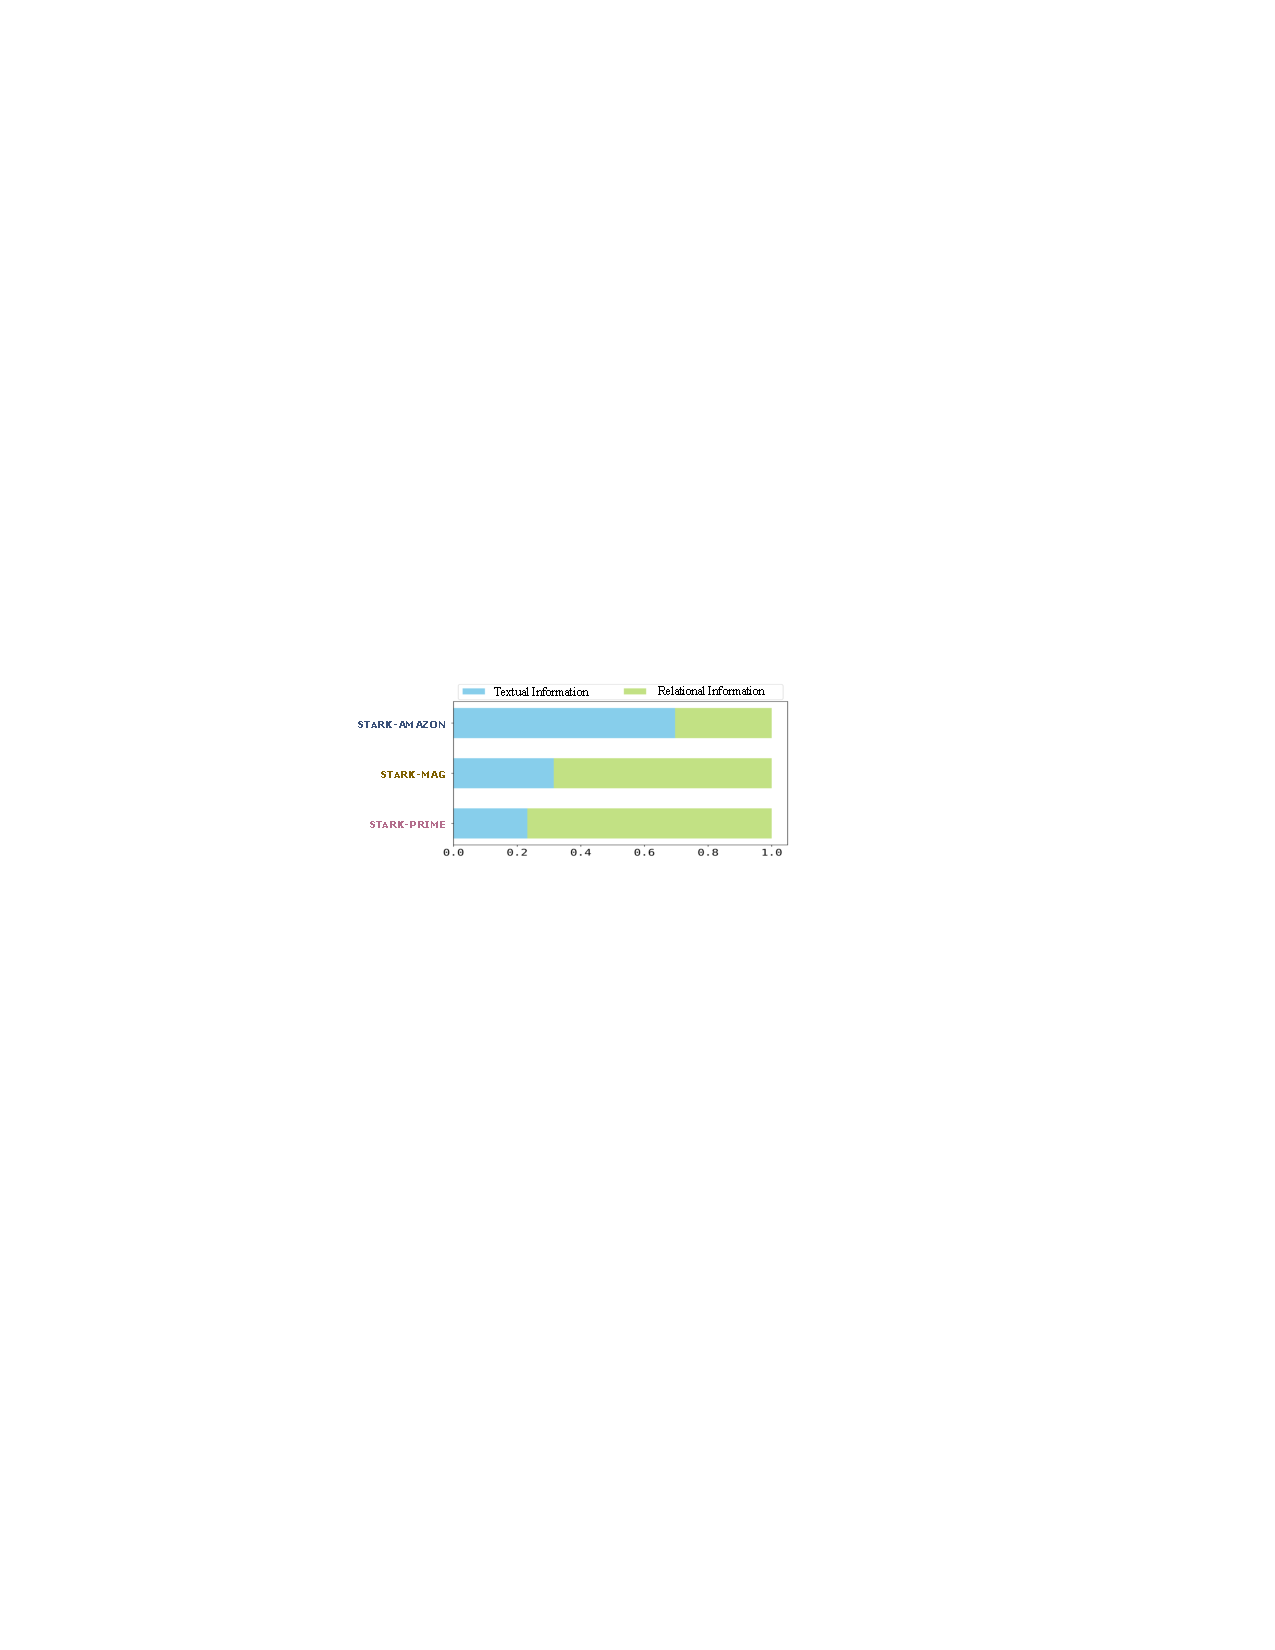
\includegraphics[width=\textwidth]{figs/ratiov2}
        \label{fig:ratio}
    \end{minipage}
    \vspace{-20pt}
\end{figure}


\subsection{Synthesized Data Distribution Analysis and Human Evaluation}
\label{sec:analysis}


% We conduct analysis and human evaluation on our synthesized datasets across three dimensions.
% to understand their characteristics and assess benchmark quality through human evaluation.
\begin{itemize}[leftmargin=*]
    \item \xhdr{Query and Answer Length} 
    Query length (in words) reflects the amount of user-provided context information, while the number of answers indicates query ambiguity/concreteness.
    Figure~\ref{fig:length_dist} shows similar query length distributions across the datasets, with most queries around 16 words. Longer queries (up to 50 words) often mention other entities or provide detailed context. Notably, 
    \amazonh has a significant long-tail pattern, with about 22\% of the answers have more than 30 entities, reflecting diverse e-commerce recommendations and ambiguous user queries.
    % , which results in a higher average answer length in 
    % Table~\ref{tab:benchmark_stats}
     
    \item \xhdr{Query Diversity} %  and Answer Coverage
    A diverse set of queries poses challenges for broader applicability to meet varying user demands. We measure query diversity using Shannon Entropy for word distribution and Type-Token Ratio (TTR) for unique words. Higher values indicate greater lexical diversity. Table~\ref{tab:q_diversity} shows high Shannon Entropy and steady TTR across all datasets. For reference, we compute these metrics for the Wikipedia page of Barack Obama\footnote{\url{https://en.wikipedia.org/wiki/Barack\_Obama}}. 
    
    \item \xhdr{Proportionality of Relational \textit{vs.}Textual Information}
    Our benchmark queries feature the composition of textual and relational information. To understand the distribution of information types, we calculate the average ratio of relational to textual requirements by word count in the queries across each dataset.  
    Note that the ratios do not directly reflect their importance in determining final answers. Figure~\ref{fig:ratio} shows varying ratios, which highlights different emphases on textual versus relational requirements and challenges retrieval systems to adapt to different distributions.

\end{itemize}

\xhdr{Human evaluation} 
We qualitatively assess sampled queries from our benchmark for naturalness (resembling natural conversation), diversity (covering various question structures and complexities), and practicality (relevance to real-world situations) with 63 participants. Evaluation results, converted from a 5-point Likert-like scale to a positive/tie/negative scale, show positive and non-negative rates in Table~\ref{tab:human} (Appendix~\ref{app:exp}). On average, 94.1\%, 85.3\%, and 89.4\% of participants rated the queries neutral or above in naturalness, diversity, and practicality, respectively. These results validate the quality of our benchmark and its potential for diverse and realistic retrieval tasks.

\subsection{\revision{Benchmark Construction: Human-Generated Queries}}
\label{sec:human_generated}
To enhance our benchmark's practical relevance, we engaged 31 participants (22 native English speakers) to generate 263 queries across three SKBs following the detailed instructions (Appendix~\ref{app:instruction}) along with our interactive platform. We manually verified and filtered the ground truth answers to ensure the answer correctness. Table~\ref{tab:benchmark_stats} shows the statistics of the human-generated datasets. Finally, we analyzed the commonalities and differences between synthesized and human-generated queries. 


% To enhance the practical relevance of our benchmark dataset, we engaged 31 participants, 22 of whom are native English speakers, to generate a total of 274 queries across three SKBs. The participants were given a list of entity IDs, randomly selected from the entire entity set. They followed detailed instructions (see Appendix~\ref{app:instruction}) using our interactive platform to explore the SKB data. Subsequently, we manually filtered the ground truth answers, ensuring their accuracy through human verification. We then analyze the commonality and difference between synthesized and human-generated queries.


\begin{table}[h]
\centering
\vspace{-13pt}
\caption{Comparison of Human-generated and Synthesized Queries}
\label{tab:comparison_queries}
\begin{tabularx}{\textwidth}{|c|X|X|}
\hline
\footnotesize \textbf{Query Type} & \footnotesize \textbf{Human-generated Query} & \footnotesize \textbf{Synthesized Query} \\
\hline
\footnotesize Short and Direct & \footnotesize \textit{Red sweatshirt for proud Montreal Canadiens} & \footnotesize \textit{Suggestions for a Suunto bike mount?} \\
\hline
\makecell{\footnotesize Specific \\ \footnotesize Author \& Field}  & \textit{\footnotesize \makecell[l]{Find me papers that discuss improving\\ condenser performance authored by \\Stojan Hrnjak}} & \textit{\footnotesize \makecell[l]{Show me papers by Seung-Hyeok Kye that \\discuss separability criteria.}} \\
\hline
\footnotesize \multirow{6}{*}{Complex Context} & \textit{\footnotesize Help me. I am trying to diagnose a patient with persistent joint pain, and I suspect a condition where the bone is dying due to compromised blood supply, often linked to factors like steroid use, ... what's the name of this \textbf{sneaky bone-killing culprit}?} & \textit{\footnotesize I'm experiencing joint pain accompanied by swelling... I'm concerned about medications aggravating my fuzzy eyesight and potential blood clotting complications. Could you recommend treatments while minimizing these side effects?} \\
\hline
\end{tabularx}
\vspace{-6pt}
\end{table}




\xhdr{Commonality}
The number of answers of synthesized and human-generated queries are comparable, indicating a similar level of query ambiguity. Moreover, we observe that most styles of human-generated queries are covered in the synthesized dataset. For example, Table~\ref{tab:comparison_queries} highlights their similarities in short product queries, specific author/field inquiries, and complex contextual queries.

\xhdr{Difference}
We find that human-generated queries often exhibit more unique expressions compared to synthesized ones, such as "\textit{Give me a \textbf{fat cross} and road tire that works with my Diamondback bicycle tube}" and "\textbf{\textit{this sneaky bone-killing culprit}}". This discovery suggests a future direction for our benchmark to incorporate modern and dynamic language nuances.



\vspace{-2pt}
\section{Experiments}
\label{sec:exp}
\vspace{-2pt}

% In this section, we aim to explore the following questions:
% \begin{itemize}[leftmargin=12pt]
% \item \textbf{Q1}: How well do current retrieval approaches perform on our benchmark datasets?
% \item \textbf{Q2}: What challenges are revealed by the experiments, and more importantly, what are the potential future directions for improvement?
% \end{itemize}


% \begin{itemize}[leftmargin=*]
%     \item \xhdr{Vector Similarity Search (ada-002)} 
%     ada-002 embeds the query and the concatenated textual and relational information of each candidate entity, then computes similarity scores between query and candidate embeddings. We use OpenAI's \texttt{text-embedding-ada-002} model for generating embeddings.

%     \item \xhdr{Multi-Vector Similarity Search (multi-ada-002)}
%     It represents each entity with multiple embeddings from chunks of its textual and relational information. We compute similarities between the query and chunk embeddings, then aggregate them by averaging the top-$k$ values as the final similarity.

%     \item \xhdr{Finetuned DPR} We finetunes query and document encoders using training query-answer pairs, optimizing with contrastive loss. Positive pairs are training questions and their ground truth answers; 20 hard negatives are top false positives from ada-002. We use \texttt{roberta-base} and finetune on the entire training split for each dataset.

%     \item \textbf{QAGNN}~\cite{qagnn}. 
%     QAGNN constructs a graph with nodes from candidate entities and entities mentioned in the question, including their neighbors for a rich context. It integrates semantic embeddings from a language model, jointly modeling relational and semantic information for retrieval.

%     \item \textbf{LLM Reranker}~\cite{abs-2306-04757, abs-2310-14122}. 
%     It improves the precision of the top-$k$ ada-002 results by reranking them with LLMs. We use GPT-4-turbo (\texttt{gpt-4-1106-preview}) and Claude3 (\texttt{claude-3-opus}), setting $k=20$ for synthesized and $k=10$ for human-generated queries. Given a query, the LLMs assign each candidate entity a satisfaction score from 0 to 1 based on their textual and relational information. 
%     We evaluate on a random 10\% sample of testing queries due to high retrieval costs.
%     \vspace{-5pt}
% \end{itemize}
\subsection{Baseline Retrieval Models and Evaluation Metrics}

We extensively evaluate five classes of retrieval models described below.
\vspace{-5pt}
\begin{itemize}[leftmargin=*]
    \vspace{-1pt}   
    \item \textbf{Sparse Retriever}: \textbf{BM25}~\cite{bm25} is a traditional yet powerful sparse retrieval method based on term frequency-inverse document frequency (TF-IDF). It computes relevance scores by considering the frequency of query terms in documents, adjusted for term rarity and document length.
    
    \vspace{-1pt}   
    \item \textbf{Small Dense Retrievers}: \textbf{DPR}~\cite{dpr}, \textbf{ANCE}~\cite{ance}, and \textbf{QAGNN}~\cite{qagnn}. These compact models generate dense embeddings for both queries and documents, computing retrieval scores based on embedding similarities. They serve as baselines for comparison with LLM-based dense retrievers.
    
    \vspace{-1pt}   
    \item \textbf{LLM-based Dense Retrievers}: \textbf{text-embedding-ada-002 (abbrev. ada-002)}~\cite{oai}, \textbf{voyage-large-2-instruct (abbrev. voyage-l2-instruct)}~\cite{voyage}, \textbf{LLM2Vec-Meta-Llama-3-8B-Instruct-mntp (abbrev. LLM2Vec)}~\cite{llm2vec}, and \textbf{GritLM-7b}~\cite{GritLM}. These models leverage LLMs to generate dense embeddings that are more contextually expressive.
    
    \vspace{-1pt}   
    \item \textbf{Multivector Retrievers}: \textbf{multi-ada-002}~\cite{oai} and \textbf{ColBERTv2}~\cite{ColBERTv2}. Beyond ada-002 which represents a document as an embedding, \textbf{multi-ada-002} splits each document into overlapping chunks and embeds them using the same encoder as the query. Similarity scores between the query and chunks are aggregated using the average of the top-3 similarities, which we found to perform best. \textbf{ColBERTv2} represents each document as multiple token-level embeddings for fine-grained matching, capturing richer semantic information.
    
    \vspace{-1pt}   
    \item \textbf{LLM Rerankers}: \textbf{Claude3} and \textbf{GPT-4} rerankers~\cite{abs-2306-04757, abs-2310-14122}. These models improve the precision of top-$k$ ada-002 results by reranking them using large language models. We employ GPT-4-turbo (\texttt{gpt-4-1106-preview}) and Claude3 (\texttt{claude-3-opus}), setting $k=20$ for synthesized queries and $k=10$ for human-generated queries. Given a query, the LLMs assign a satisfaction score from 0 to 1 to each candidate entity based on textual and relational information. Due to high computational costs, we evaluate these rerankers on a random 10\% sample of test queries.
\end{itemize}

The performance of these models are measured using standard retrieval metrics below.

% We use metrics including Hit@1, Hit@5, Mean Reciprocal Rank (MRR), and Recall@20. See Appendix~\ref{app:metrics} for details.

% \subsection{Evaluation Metrics}
% \label{app:metrics}

% We use the following metrics to holistically evaluate the model performance.

\vspace{-5pt}
\begin{itemize}[leftmargin=*]

    \vspace{-1pt}   
    \item \textbf{Hit@$k$} assesses whether the correct item is among the top-$k$ results from the model. We used $k=1$ and $k=5$ for evaluation. At $k=1$, it evaluates the accuracy of the top recommendation; at $k=5$, it examines the model's precision in a wider recommendation set.  
    % It's a straightforward yet effective way to measure the immediate relevance of answers.

    \vspace{-1pt}   
    \item \textbf{Recall@$k$} measures the proportion of relevant items in the top-$k$ results. For synthesized queries, $k=20$ is used, as the answer length of all of the queries in our benchmarks are equal or smaller then $20$. 
    % For human-generated queries, Recall@20 is not reported as the number of responses in the human-generated subset may exceed 20. 
    This metric offers insight into the model's ability to identify all relevant items, particularly in scenarios where missing any could be critical. 

    \vspace{-1pt}   
    \item \textbf{Mean Reciprocal Rank (MRR)} is a statistic for evaluating the average effectiveness of a predictive model. It calculates the reciprocal of the rank at which the first relevant item appears in the list of predictions. 
    % MRR is particularly useful for understanding the model's performance at presenting the correct item at an early stage, without the need for a predefined $k$. 
    This metric emphasizes the importance of the rank of the first correct answer, which is crucial in many practical applications where the first correct answer is often the most impactful.
\end{itemize}

\subsection{Results and Analysis}
\vspace{-2pt}

% \begin{table}[htbp]
%     \centering
%     \resizebox{1.0\textwidth}{!}{
%     \begin{tabular}{l|cccc|cccc|cccc}
%         \toprule
%         & \multicolumn{4}{c|}{\amazont} & \multicolumn{4}{c|}{\magt} & \multicolumn{4}{c}{\primekgt} \\
%         & \textbf{\small Hit@1} & \textbf{\small Hit@5} & \textbf{\small Recall@20} & \textbf{\small MRR} & \textbf{\small Hit@1} & \textbf{\small Hit@5} & \textbf{\small Recall@20} & \textbf{\small MRR} & \textbf{\small Hit@1} & \textbf{\small Hit@5} & \textbf{\small Recall@20} & \textbf{\small MRR}  \\
%         \midrule
%         % \textbf{RAG-Base} &0.0673& 0.1561 & 0.1233 &0.1373  &0.0349&0.0513 & 0.0555& 0.0369& 0.0324 & 0.0834& 0.1008 & 0.0588 \\
%         \textbf{Dense Retriever (\texttt{roberta})}        & 0.1529 & 0.4793& 0.4449&0.3020&&&\\
%         \textbf{QAGNN (\texttt{roberta})}        &&&&\\
%         \textbf{VSS (\texttt{ada-002})}        & 0.3916 & 0.6273 & 0.5329 & 0.5035 & 0.2908 & 0.4961 & 0.4836 & 0.3862 & 0.1263 & 0.3149 & 0.3600 & 0.2141\\
%         \textbf{MultiVSS (\texttt{ada-002})} & 0.4007 & 0.6498 & 0.5512 & 0.5155 & 0.2592 & 0.5043 & 0.5080 & 0.3694 & 0.1510 & 0.3356 & 0.3805 & 0.2349\\
%         % \textbf{RAG-FT} &0.2026 & 0.3037 & 0.3969  & 0.2340  &0.0361 &0.0482 & 0.0627&0.0442& 0.0370 &0.0867 & 0.1359 & 0.0618\\
%         \textbf{VSS+Claude Reranker}   & 0.4266 & 0.6746 & 0.5376 & 0.5329 & 0.3202& 0.5334&  0.4834& 0.4129& 0.1611 & 0.3582 & 0.3598 & 0.2466\\
%         \textbf{VSS+GPT4 Reranker}   & 0.4479 & 0.7117 & 0.5535 & 0.5569 &0.4090 &0.5818 &0.4860 & 0.4900& 0.1828 & 0.3728&0.3405 & 0.2655\\
%         \bottomrule
%     \end{tabular}
%         }
%     \label{tab:results}
%     \caption{Main experimental results. Last row shows the relative improvements over the best metric value among the baselines.}
% \end{table}


% \begin{table}[htbp]
%     \centering
%     \resizebox{1.0\textwidth}{!}{
%     \begin{tabular}{l|cccc|cccc|cccc}
%         \toprule
%         & \multicolumn{4}{c|}{\amazont} & \multicolumn{4}{c|}{\magt} & \multicolumn{4}{c}{\primekgt} \\
%         & \textbf{\small Hit@1} & \textbf{\small Hit@5} & \textbf{\small Recall@20} & \textbf{\small MRR} & \textbf{\small Hit@1} & \textbf{\small Hit@5} & \textbf{\small Recall@20} & \textbf{\small MRR} & \textbf{\small Hit@1} & \textbf{\small Hit@5} & \textbf{\small Recall@20} & \textbf{\small MRR}  \\
%         \midrule
%         \textbf{Dense Retriever (\texttt{roberta})}        & 0.1529 & 0.4793& 0.4449&0.3020&&&\\
%         \textbf{QAGNN (\texttt{roberta})}        &&&&\\
%         \textbf{VSS (\texttt{ada-002})}        & 0.3916 & 0.6273 & 0.5329 & 0.5035 & 0.2908 & 0.4961 & 0.4836 & 0.3862 & 0.1263 & 0.3149 & 0.3600 & 0.2141\\
%         \textbf{MultiVSS (\texttt{ada-002})} & 0.4007 & 0.6498 & 0.5512 & 0.5155 & 0.2592 & 0.5043 & 0.5080 & 0.3694 & 0.1510 & 0.3356 & 0.3805 & 0.2349\\
%         \textbf{VSS+Claude Reranker}   & 0.4266 & 0.6746 & 0.5376 & 0.5329 & 0.3202& 0.5334&  0.4834& 0.4129& 0.1611 & 0.3582 & 0.3598 & 0.2466\\
%         \textbf{VSS+GPT4 Reranker}   & 0.4479 & 0.7117 & 0.5535 & 0.5569 &0.4090 &0.5818 &0.4860 & 0.4900& 0.1828 & 0.3728&0.3405 & 0.2655\\
%         \bottomrule
%     \end{tabular}
%         }
%     \label{tab:results}
%     \caption{Main experimental results. Last row shows the relative improvements over the best metric value among the baselines.}
% \end{table}

% submit
% \begin{table}[t]
%     \centering
%     \vspace{-10pt}
%     \caption{\textbf{Testing results on \benchmarkt-Syn(thesized).} (*) indicates partial evaluation (on random 10\% of the test queries) due to the high latency and cost of the methods. }
%     \resizebox{0.9\textwidth}{!}{
%     \begin{tabular}{l|lcccccc}
%         \toprule
%         && \textbf{\small Dense Retriever} & \textbf{\small QAGNN } & \textbf{\small VSS} & \textbf{\small MultiVSS} & \textbf{*\small Claude3} & \textbf{*\small GPT4} \\
%         &&{\small\texttt{(roberta)}} &{\small\texttt{(roberta)}}&{\small \texttt{(ada-002)}}&{\small \texttt{(ada-002)}}& \textbf{\small Reranker} & \textbf{\small Reranker}\\
%         \midrule
%         \multirow{4}{*}{\textbf{\small \amazont}}&Hit@1    & 0.1529 & 0.2656 & 0.3916 & 0.4007 & \textbf{0.4549} & 0.4479 \\
%         &Hit@5    & 0.4793 & 0.5001 & 0.6273 & 0.6498 & 0.7113 & \textbf{0.7117} \\
%         &Recall@20& 0.4449 & 0.5205 & 0.5329 & 0.5512 & 0.5377 & \textbf{0.5535} \\
%         &MRR      & 0.3020 & 0.3775 & 0.5035 & 0.5155 & \textbf{0.5591} & 0.5569 \\
%         \midrule
%         \multirow{4}{*}{\textbf{\small\magt}}&Hit@1    &0.1051 & 0.1288 & 0.2908 & 0.2592 & 0.3654 & \textbf{0.4090} \\
%         &Hit@5    &0.3523 & 0.3901 & 0.4961 & 0.5043 & 0.5317 & \textbf{0.5818} \\
%         &Recall@20& 0.4211 & 0.4697 & 0.4836 & \textbf{0.5080} & 0.4836 & 0.4860 \\
%         &MRR      & 0.2134 & 0.2912 & 0.3862 & 0.3694 & 0.4415 & \textbf{0.4900} \\
%         \midrule
%         \multirow{4}{*}{\textbf{\small\primekgt}} &Hit@1    &0.0446 & 0.0885 & 0.1263 & 0.1510 & 0.1779 &\textbf{ 0.1828} \\
%         &Hit@5    &0.2185 & 0.2135 & 0.3149 & 0.3356 & 0.3690 & \textbf{0.3728} \\
%         &Recall@20 & 0.3013 & 0.2963 & 0.3600 & \textbf{0.3805} & 0.3557 & 0.3405 \\
%         &MRR &0.1238 & 0.1473 & 0.2141 & 0.2349 & 0.2627 & \textbf{0.2655} \\
%         \bottomrule
%     \end{tabular}
%     }
%     \vspace{-15pt}
%     \label{tab:results}
% \end{table}

\begin{table}[t]
    \centering
    \vspace{-10pt}
    \caption{Testing results on \benchmarkt-Syn(thesized).}
    \resizebox{1.0\textwidth}{!}{
    \begin{tabular}{r|rrrr|rrrr|rrrr}
        \toprule
        & \multicolumn{4}{c|}{\amazont} & \multicolumn{4}{c|}{\magt} & \multicolumn{4}{c}{\primekgt} \\
         & Hit@1 & Hit@5 & R@20 & MRR & Hit@1 & Hit@5 & R@20 & MRR & Hit@1 & Hit@5 & R@20 & MRR \\
        \hline
        \rowcolor{cyan!10} \multicolumn{13}{c}{\textbf{Full Testing Dataset}} \\
        \hline
        BM25 & 44.94 & \textbf{67.42} & 53.77 & 55.30 & 25.85 & 45.25 & 45.69 & 34.91 & 12.75 & 27.92 & 31.25 & 19.84 \\
        DPR (roberta) & 15.29 & 47.93 & 44.49 & 30.20 & 10.51 & 35.23 & 42.11 & 21.34 & 4.46 & 21.85 & 30.13 & 12.38 \\
        ANCE (roberta) & 30.96 & 51.06 & 41.95 & 40.66 & 21.96 & 36.50 & 35.32 & 29.14 & 6.53 & 15.67 & 16.52 & 11.05 \\
        
        QAGNN (roberta) & 26.56 & 50.01 & 52.05 & 37.75 & 12.88 & 39.01 & 46.97 & 29.12 & 8.85 & 21.35 & 29.63 & 14.73 \\
        ada-002 & 39.16 & 62.73 & 53.29 & 50.35 & 29.08 & 49.61 & 48.36 & 38.62 & 12.63 & 31.49 & 36.00 & 21.41 \\
        % VSS (oai-3-large) & - & - & - & - & 38.04 & 61.50 & 59.03 & 48.95 & 16.32 & 38.52 & 45.51 & 26.63 \\
        voyage-l2-instruct & 40.93 & 64.37 & 54.28 & 51.60 & 30.06 &  50.58 & \textbf{50.49} & 39.66 & 10.85 & 30.23 & 37.83 & 19.99 \\ 
        LLM2Vec & 21.74 & 41.65 & 33.22 & 31.47 & 18.01 & 34.85 & 35.46 & 26.10 & 10.10 & 22.49 & 26.34 & 16.12 \\
        GritLM-7b & 42.08 & 66.87 & \textbf{56.52} & 53.46 & \textbf{37.90} & \textbf{56.74} & 46.40 & \textbf{47.25} & \textbf{15.57} & 33.42 & \textbf{39.09} & \textbf{24.11} \\
        multi-ada-002 & 40.07 & 64.98 & 55.12 & 51.55 & 25.92 & 50.43 & 50.80 & 36.94 & 15.10 & \textbf{33.56} & 38.05 & 23.49 \\
        ColBERTv2 & \textbf{46.10} & 66.02 & 53.44 & \textbf{55.51} & 31.18 & 46.42 & 43.94 & 38.39 & 11.75 & 23.85 & 25.04 & 17.39 \\
        \hline
        \rowcolor{green!8} \multicolumn{13}{c}{\textbf{Random 10\% Sample}} \\
        \hline
        BM25 & 42.68 & 67.07 & 54.48 & 54.02 & 27.81 & 45.48 & 44.59 & 35.97 & 13.93 & 31.07 & 32.84 & 21.68 \\
        DPR (roberta) & 16.46 & 50.00 & 42.15 & 30.20 & 11.65 & 36.84 & 42.30 & 21.82 & 5.00 & 23.57 & 30.50 & 13.50 \\
        ANCE (roberta) & 30.09 & 49.27 & 41.91 & 39.30 & 22.89 & 37.26 &44.16 & 30.00 & 6.78 & 16.15 & 17.07 & 11.42 \\
        QAGNN (roberta) & 25.00 & 48.17 & 51.65 & 36.87 & 12.03 & 37.97 & 47.98 & 28.70 & 7.14 & 17.14 & 32.95 & 16.27 \\
        ada-002 & 39.02 & 64.02 & 49.30 & 50.32 & 28.20 & 52.63 & 49.25 & 38.55 & 15.36 & 31.07 & 37.88 & 23.50 \\
        voyage-l2-instruct & 43.29 & 67.68 & 56.04 & 54.20 & 34.59 & 50.75 & 50.75 & 42.90 & 12.14 & 31.42 & 37.34 & 21.23 \\
        LLM2Vec & 18.90 & 37.80 & 34.73 & 28.76 & 19.17 & 33.46 & 29.85 & 26.06 & 9.29 & 20.7 & 25.54 & 15.00 \\
        GritLM-7b & 43.29 & \textbf{71.34} & \textbf{56.14} & 55.07 & 38.35 & \textbf{58.64} & 46.38 & 48.25 & 16.79 & 34.29 & 41.11 & 24.99 \\
        % VSS (oai-3-large) & - & - & - & - & - & - & - & - & - & - & - & - \\
        multi-ada-002 & 40.85 & 62.80 & 52.47 & 51.54 & 25.56 & 50.37 & \textbf{53.03} & 36.82 & 15.36 & 32.86 & \textbf{40.99} & 23.70 \\
        ColBERTv2 & 44.31 & 65.24 & 51.00 & 55.07 & 31.58 & 47.36 & 45.72 & 38.98 & 15.00 & 26.07 & 27.78 & 19.98 \\
        Claude3 Reranker & \textbf{45.49} & 71.13 & 53.77 & \textbf{55.91} & 36.54 & 53.17 & 48.36 & 44.15 & 17.79 & 36.90 & 35.57 & 26.27 \\
        GPT4 Reranker & 44.79 & 71.17 & 55.35 & 55.69 & \textbf{40.90} & 58.18 & 48.60 & \textbf{49.00} & \textbf{18.28} & \textbf{37.28} & 34.05 & \textbf{26.55} \\
        \bottomrule
    \end{tabular}
    }
    \label{tab:results}
\end{table}


% \begin{table}[h]
%     \centering
%     \vspace{-15pt}
%     \caption{Testing results on \benchmarkt-Human(-Generated).}
%     \resizebox{0.85\textwidth}{!}{
%     \begin{tabular}{l|lcccc}
%         \toprule
%         & & \textbf{\small VSS} & \textbf{\small MultiVSS} & \textbf{\small Claude3} & \textbf{\small GPT4} \\
%         & & {\small \texttt{(ada-002)}}&{\small \texttt{(ada-002)}}& \textbf{\small Reranker} & \textbf{\small Reranker}\\
%         \midrule
%         \multirow{3}{*}{\textbf{\small \amazont}}
%         &Hit@1    & 0.3950 & 0.4691 & \textbf{0.5602} & 0.5432 \\
%         &Hit@5    & 0.6419 & \textbf{0.7284} & \textbf{0.7284} & \textbf{0.7284}\\
%         &Recall@20    & 0.3546 & \textbf{0.4022} & 0.3546 & 0.3546 \\\
%         &MRR      & 0.5265 & 0.5874 & \textbf{0.6439} & 0.6274\\
%         \midrule
%         \multirow{3}{*}{\textbf{\small\magt}}
%         &Hit@1    & 0.2857 & 0.2381 & \textbf{0.3810} & 0.3690 \\
%         &Hit@5    & 0.4167 & 0.4167 & \textbf{0.4643} & 0.4523\\
%         % &Recall@20& & & & \\
%         &Recall@20    & 0.3595 & \textbf{0.3985} & 0.3595 & 0.3595\\
%         &MRR      & 0.3581 & 0.3143 & \textbf{0.4243} & 0.4031\\
%         \midrule
%         \multirow{3}{*}{\textbf{\small\primekgt}} 
%         &Hit@1    & 0.2120 & 0.2567 & \textbf{0.2844} & \textbf{0.2844}\\
%         &Hit@5    & 0.4037 & 0.4037 & 0.4771 & \textbf{0.4863} \\
%         &Recall@20    & 0.4383 & \textbf{0.4979} & 0.4383  & 0.4383 \\
%         % &Recall@20 & & & & \\
%         &MRR      & 0.2984 & 0.3377 & \textbf{0.3623} & 0.3617 \\
%         \bottomrule
%     \end{tabular}
%     }
%     \label{tab:results-human}
% \end{table}

\begin{table}[t]
    \centering
    \vspace{-10pt}
    \caption{Testing results on \benchmarkt-Human(-Generated).}
    \resizebox{1.0\textwidth}{!}{
    \begin{tabular}{r|rrrr|rrrr|rrrr}
        \toprule
        & \multicolumn{4}{c|}{\textbf{\amazont}} & \multicolumn{4}{c|}{\textbf{\magt}} & \multicolumn{4}{c}{\textbf{\primekgt}} \\
        Method & Hit@1 & Hit@5 & R@20 & MRR & Hit@1 & Hit@5 & R@20 & MRR & Hit@1 & Hit@5 & R@20 & MRR \\
        \midrule
        BM25 & 27.16 & 51.85 & 29.23 & 18.79 & 32.14 & 41.67 & 32.46 & 37.42 & 22.45 & 41.84 & 42.32 & 30.37 \\
        DPR (roberta) & 16.05 & 39.51 & 15.23 & 27.21 & 4.72 & 9.52 & 25.00 & 7.90 & 2.04 & 9.18 & 10.69 & 7.05 \\
        ANCE (roberta) &25.93 & 54.32 & 23.69 & 37.12 & 25.00 & 30.95 & 27.24 & 27.98 & 7.14 & 13.27 & 11.72 & 10.07 \\
        QAGNN (roberta) & 22.22 & 49.38 & 21.54 & 31.33 & 20.24 & 26.19 & 28.76 & 25.53 & 6.12 & 13.27 & 17.62 & 9.39 \\
        ada-002 & 39.50 & 64.19 & 35.46 & 52.65 & 28.57 & 41.67 & 35.95 & 35.81 & 17.35 & 34.69 & 41.09 & 26.35 \\
        voyage-l2-instruct & 35.80 & 62.96 & 33.01 & 47.84 & 22.62 & 36.90 & 32.44 & 29.68 & 16.33 & 32.65 & 39.01 & 24.33 \\
        LLM2Vec & 29.63 & 46.91 & 21.21 & 38.61 & 16.67 & 28.57 & 21.74 & 21.59 & 9.18 & 21.43 & 26.77 & 15.24 \\
        GritLM-7b & 40.74 & 71.60 & 36.30 & 53.21 & 34.52 & 44.04 & 34.57 & 38.72 & 25.51 & 41.84 & \textbf{48.10} & 34.28 \\ 
        multi-ada-002 & 46.91 & 72.84 & \textbf{40.22} & 58.74 & 23.81 & 41.67 & \textbf{39.85} & 31.43 & 24.49 & 39.80 & 47.21 & 32.98 \\
        ColBERTv2 & 33.33 & 55.56 & 29.03 & 43.77 & 33.33 & 36.90 & 30.50 & 35.97 & 15.31 & 26.53 & 25.56 & 19.67 \\
        Claude3 Reranker & \textbf{53.09} & 74.07 & 35.46 & \textbf{62.11} & \textbf{38.10} & 45.24 & 35.95 & \textbf{42.00} & \textbf{28.57} & \textbf{46.94} & 41.61 & \textbf{36.32} \\
        GPT4 Reranker & 50.62 & \textbf{75.31} & 35.46 & 61.06 & 36.90 & \textbf{46.43} & 35.95 & 40.65 & \textbf{28.57} & 44.90 & 41.61 & 34.82 \\
        \bottomrule
    \end{tabular}
    }
    \label{tab:results-human}
    \vspace{-10pt}
\end{table}



\textbf{Results on synthesized queries.} 
Table~\ref{tab:results} presents the results on both the full synthesized test sets and random 10\% samples from these sets. In both cases, \textbf{BM25}, despite its simplicity, proves to be a strong baseline, outperforming the dense retrieval models such as \textbf{ANCE}. We observe that finetuned \textbf{DPR} and \textbf{QAGNN}, exhibit insufficient performance. This underperformance is likely due to their relatively small model sizes and the risk of overfitting during training. These issues present challenges in effectively training the models on SKBs, where the entity documents can be hard to differentiate without capturing detailed information.

Among the larger models, \textbf{ada-002} benefits from superior pretrained embeddings and significantly outperforms \textbf{LLM2Vec} by a large margin. \textbf{GritLM-7b} delivers excellent performance, surpassing the ada-002 model overall. In contrast, LLM2Vec underperforms due to its limited context length, which is insufficient for encoding the lengthy documents in the SKBs. For multivector retrievers, we found that \textbf{multi-ada-002} generally outperforms ada-002, indicating that using multiple vectors per document enhances retrieval effectiveness. Similarly, fine-grained representation allows \textbf{ColBERTv2} to capture subtle semantic nuances between queries and documents, leading to largely improved retrieval accuracy. 

However, both GritLM-7b and ColBERTv2 generally underperform compared to the rerankers on the random split, especially in terms of Hit@k metrics. This suggests that while these dense retriever models effectively capture semantic information, they may not fully grasp the nuanced relevance judgments required for top-tier retrieval performance. The rerankers, utilizing powerful LLMs like \textbf{GPT-4 (gpt-4-1106-preview)} and \textbf{Claude3 (claude-3-opus)}, excel by re-evaluating the top candidates and assigning satisfaction scores based on a deeper understanding of the query and document content. This process allows them to better discern subtle contextual cues and relational information that dense retrievers might overlook. Consequently, LLM rerankers enhance retrieval precision at the top ranks.

Finally, regardless of the higher computational costs of the rerankers, their performance remains suboptimal. For instance, the Hit@1 scores for the GPT-4 reranker are only about 18\% on \primekgt and 41\% on \magt, indicating that the top-ranked answers are frequently incorrect. Similarly, the Recall@20 metrics are below 60\% across all datasets, with the GPT-4 reranker achieving Recall@20 scores of 55\% on \amazont, 49\% on \magt, and 34\% on \primekgt. This suggests that the ranking results miss a significant portion of relevant answers. The MRR scores are also relatively low, especially for \primekgt, where the GPT-4 reranker attains an MRR of only around 27\%. 

The insufficient performances may be attributed to the complexity and diversity of queries in SKBs, where nuanced understanding and detailed contextual information are crucial.
These findings highlight significant room for improvement in the ranking process.


\xhdr{Results on human-generated dataset}  
Table~\ref{tab:results-human} presents the testing results on the human-generated datasets. For example, the rerankers consistently outperform others, showing their reasoning and context understanding ability. Compared to the synthesized datasets, the performance on human-generated queries is generally higher for most models, but the overall trends remain consistent. This indicates that synthesized datasets may be more challenging, highlighting the complexity of the tasks on our synthesized queries. 

Another interesting observation is that the performance of the rerankers is particularly strong on human-generated queries, which may contain more nuanced language and diverse expressions. This suggests that rerankers excel in interpreting and leveraging the richness of human language to improve retrieval accuracy.



\begin{table}[t]
    \centering
    \caption{Latency (s) of the retrieval systems on \benchmarkt. }
    \resizebox{0.9\textwidth}{!}{
    \begin{tabular}{l|cccccc}
        \toprule
        &\textbf{\small DPR} & \textbf{\small QAGNN } & 
        \textbf{\small ada-002} & \textbf{\small multi-ada-002} & \textbf{\small Claude3 Reranker} & \textbf{\small GPT4 Reranker} \\
        \midrule
        \textbf{\amazont} & 2.34 & 2.32 &5.71 &4.87 & 27.24&24.76 \\
        \textbf{\magt} & 0.94 &1.35 &2.25 &3.14 &22.60 & 23.43 \\
        \textbf{\primekgt} & 0.92 & 1.29 &0.54 &0.90 &29.14 &26.97 \\
        \midrule 
        \textbf{Average} & 1.40  & 1.65 &2.83 &2.97 &26.33 &25.05 \\
        \bottomrule
    \end{tabular}
    }
    \label{tab:latency}
    \vspace{-10pt}
\end{table}

% On the other hand, this suggests the complexities of 
% for our benchmark and demonstrates the value of a double-checking process due to the complexities of our text and relational data requirements.


\begin{figure}[t]
    \centering
    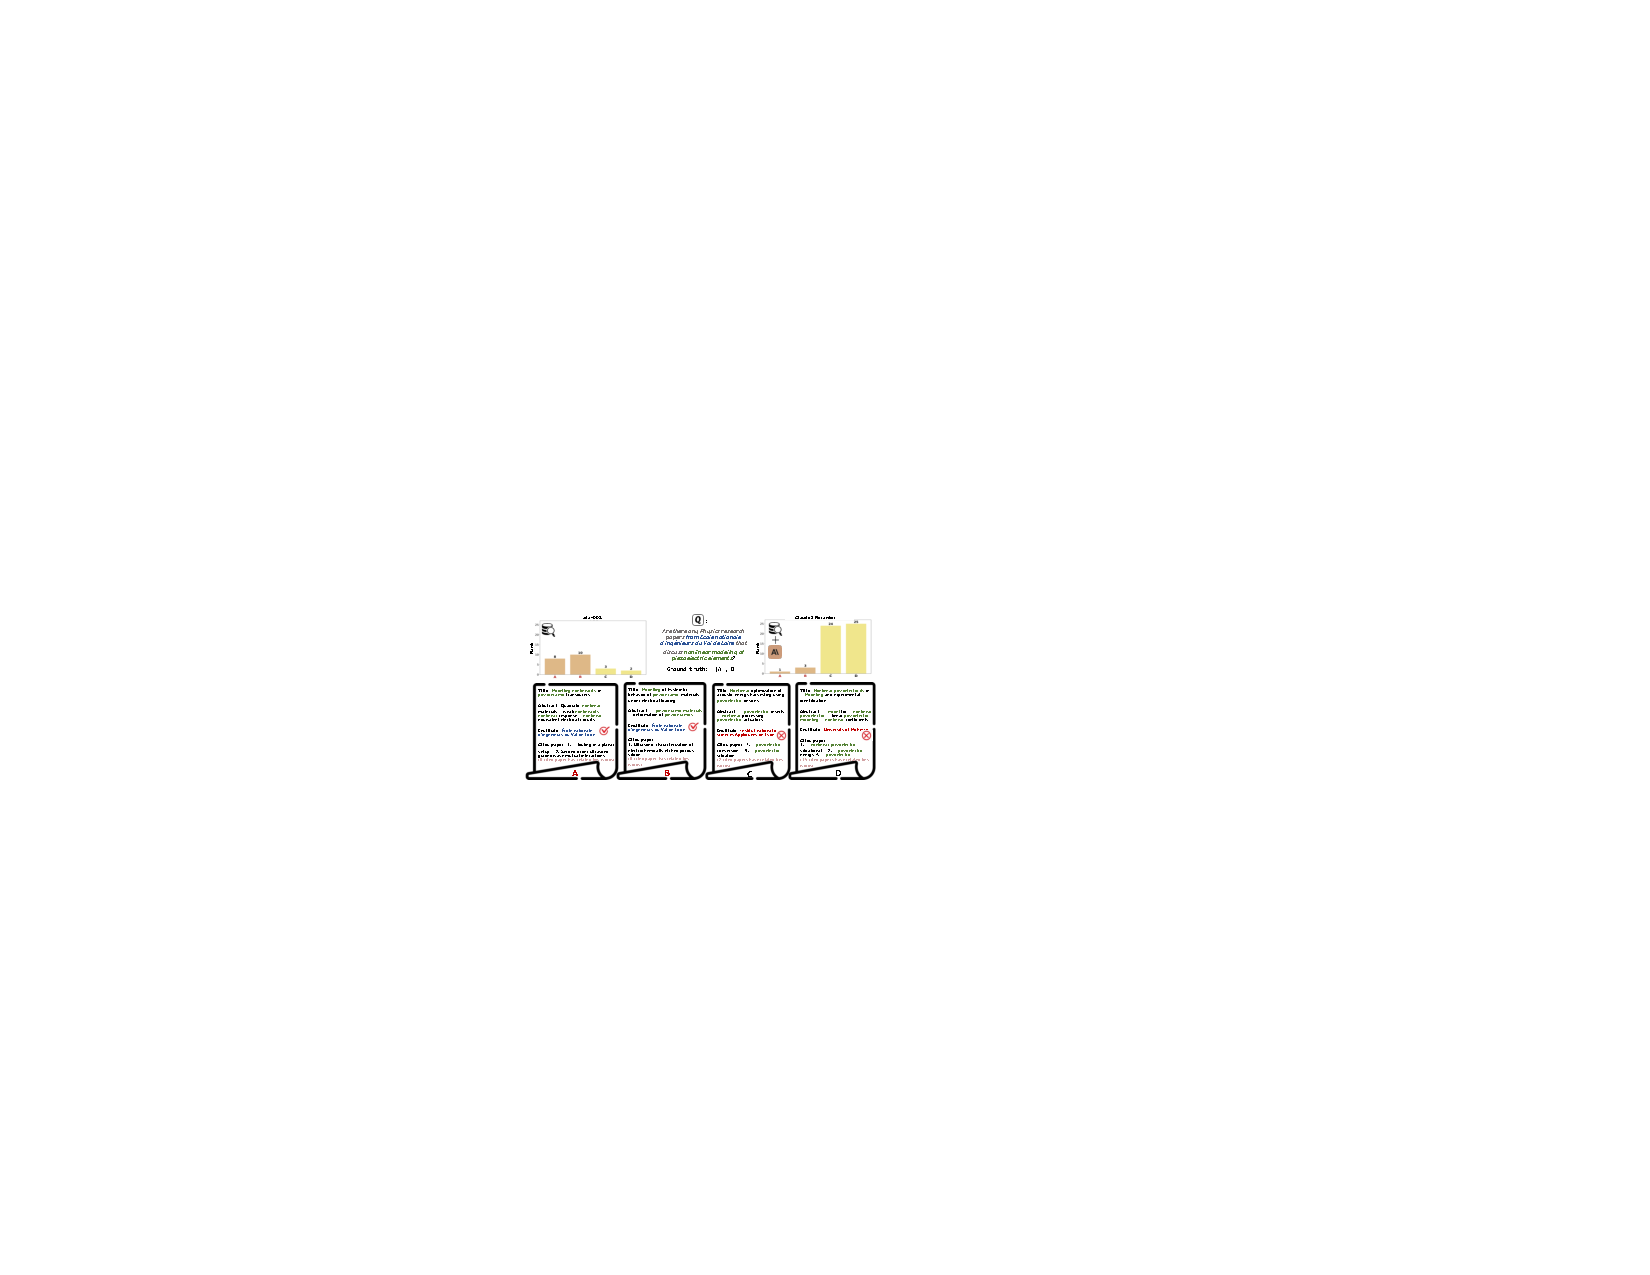
\includegraphics[width=1\textwidth]{figs/case_updated}
    \caption{
    A case study on \magh shows that ada-002 overranks non-ground truth papers $C$ and $D$ due to repeated keywords in the relational information ``cites paper''. After reranking with Claude3, it correctly prioritizes ground truth papers $A$ and $B$ with accurate reasoning and analysis.}
    \vspace{-10pt}
    \label{fig:case}
\end{figure}

\xhdr{Retrieval latency} Latency is crucial for practical retrieval systems, as users expect quick responses. As shown in Table~\ref{tab:latency}, we evaluated the latency of various models using a single NVIDIA A100-SXM4-80GB GPU. We observed that the DPR and QAGNN models exhibit lower average latency, making them suitable for time-sensitive applications. In contrast, the ada-002 and multi-ada-002 models have moderate latency due to multiple API calls. However, when combined with LLM rerankers, the latency increases significantly due to the computational demands of these large models. Therefore, it is important to balance accuracy and latency, especially for complex queries that require advanced reasoning capabilities. 


\xhdr{Case study} 
To highlight the importance of reasoning ability for achieving good performance on our benchmark, we present a case study in Figure~\ref{fig:case}, comparing the ada-002 model with the Claude3 Reranker. In this example, the query requests papers from a specific institution on a particular topic. The ada-002 model fails to address the relational aspect of the query because it embeds entire documents without detailed analysis. This leads to high relevance scores for irrelevant papers that frequently mention keywords like "nonlinear modeling" and "piezoelectric elements" but do not satisfy the relational requirement. In contrast, the LLM reranker significantly improves the results by reasoning about the relationship between the query and each paper, resulting in scores that more accurately reflect relevance. This underscores the need for reasoning ability to grasp query complexities. 


\section{Related Work}
\label{sec:related}


\begin{comment}
\xhdr{Knowledge Base Question-Answering and Retrieval}

\textbf{unstructured qa dataset:} single-document dataset: SQuAD, NewsQA, Natural Questions, MS MARCO, CoQA ; mult-document dataset: HotpotQA, TriviaQA, SearchQA,  WikiHop, QuAC

\textbf{structured qa dataset:} KGQA, use pre-existing knowledge bases with pre-defined rules to generate qa pairs, WebQuestions, WebQuestionsSP, ComplexWebQuestions~~\cite{ComplexWebQuestions}, SimpleQuestions, ComplexQuestions,  KQA Pro, MetaQA, LC-QuAD 2.0, QALD

\textbf{semi-structure qa dataset:} Only exist tabular + textual dataset.  WikiTableQuestions, Spider, WikiSQL, TabFact, HybridQA, TabMCQ


open-domain question answering tasks 

HotpotQA~~\cite{yang2018hotpotqa} feature: multi-hop reasoning, multiple supporting documents, provide sentence level supporting facts, factoid comparison questions (arithmetic comparison). Collection: human curated, crowdsourcing on wikipedia. Format: RC, no candidate set

SQuAD: single-hop reasoning, answer by single sentences matching. Collection: crowdworkers on wikipedia. Format: reading comprehension, no candidate set

TriviaQA: multiple supporting documents, supporting documents collected by information retrieval after qa pairs generated, syntactic and lexical variability. Disadvantage: answer extraction from documents Collection: from trivia qa pairs, use bing search and wiki page of relevant entities.

SearchQA: multiple supporting documents. Collection: start from existing qa pair and augment by IR by google.

MS-MARCO: system generated free-form answer evaluated by pre-defined metrics (eg. BLEU-1, ROUGE-L), have reliability issue

ComplexWebQuestions: focus on question decomposition: conjunctions, superlatives,
comparatives, and compositions,  Collection: SPARQL + mechanical turk

QA through semantic parsing has focused primarily on compositionality:
questions are translated to compositional programs that encode a sequence of actions for finding the answer in a knowledge-base (KB) 

WebQuestions: semantic parsing, KB

WikiTableQuestions: semantic parsing, complex questions on semi-structured tables 


WikiHop and MedHopo~~\cite{WelblSR18},: multi-hop reasoning


open-domain:
Structured knowledge-based QA(KB)~~\cite{BerantCFL13, YihCHG15} known as KBQA.

unstructured knowledge-based QA~~\cite{IzacardG21, realm, KarpukhinOMLWEC20, LeeCT19, YangXLLTXLL19}

UniK-QA~~\cite{UniK-QA}
SearchQA~~\cite{dunn2017searchqa}
TriviaQA~~\cite{TriviaQA}

Knowledge base question answering datasets are either limited in scale or in the complexity of questions.

WikiHop and MedHop~~\cite{WelblSR18}, ComplexWebQuestions~~\cite{ComplexWebQuestions} diversity restricted by the KB schema.
\end{comment}


% We identify three primary categories on retrieval-oriented question answering (QA) datasets 
% \shiyu{of retrieval-based question answering (QA) dataset?} \qian{of what? of retrieval system?} 
% based on the knowledge sources they utilize: unstructured, structured, and semi-structured knowledge bases. 
% Each of these categories plays a crucial role in advancing the field of information retrieval and question answering, yet they also present distinct limitations that our work seeks to address.

% \xhdr{Unstructured QA Datasets} 
% The line of work explores retrieving answers from a single document~\cite{rajpurkar-etal-2016-squad} or multiple document sources~\cite{trischler-etal-2017-newsqa, yang-etal-2018-hotpotqa, TriviaQA, WelblSR18, dunn2017searchqa}.
% For example, SQuAD~\cite{rajpurkar-etal-2016-squad} focuses on extracting answers from a single document, testing model's ability to understand and retrieve information within a specific context. For multi-document retrieval, HotpotQA~\cite{yang-etal-2018-hotpotqa} demands reasoning over multiple documents and includes sentence-level supporting facts, enhancing the complexity of the retrieval task. TriviaQA~\cite{TriviaQA} combines questions from trivia games with evidence documents, evaluating both retrieval and reasoning over multiple sources. 
% Moreover, some works~\cite{DBLP:conf/nips/NguyenRSGTMD16, kwiatkowski-etal-2019-natural} leverage generated results by search engines as ground truth answers or information sources for retrieval. 
\xhdr{Unstructured QA Datasets}
This research domain consists of methods for retrieving answers from unstructured text, either from a single document~\cite{rajpurkar-etal-2016-squad} or multiple documents~\cite{trischler-etal-2017-newsqa, yang-etal-2018-hotpotqa, TriviaQA, WelblSR18, dunn2017searchqa}. For instance, SQuAD~\cite{rajpurkar-etal-2016-squad} is designed for answer extraction within a specific document, while approaches like HotpotQA~\cite{yang-etal-2018-hotpotqa} and TriviaQA~\cite{TriviaQA} extend to multi-document contexts. Additionally, some studies utilize search engine outputs as a basis or supplementary data for question answering~\cite{DBLP:conf/nips/NguyenRSGTMD16, kwiatkowski-etal-2019-natural}.
However, unstructured QA datasets often lack the depth of relational reasoning commonly required in answering complex user queries. \revision{In contrast, \benchmarkh contains queries demanding multi-hop relational reasoning to challenge model's ability of handling structured information. }
% \jure{This is a nice summary but it does not answer how STARK differers/related to this line of work. Say: "In contrast, STARK is..." or "STARK extends this line of work by ..." or something similar.}
% Datasets like SQuAD~\cite{rajpurkar-etal-2016-squad} focus on extracting answers from a single document, testing the model's ability to understand and retrieve information within a specific context. NewsQA~\cite{trischler-etal-2017-newsqa} introduces the challenge of answering questions from news articles, emphasizing real-world applicability and information synthesis. Natural Questions~\cite{kwiatkowski-etal-2019-natural} requires answering questions based on Google search results, reflecting genuine user inquiries and web search scenarios. MS MARCO~\cite{DBLP:conf/nips/NguyenRSGTMD16} provides real-world queries with system-generated answers, aiming to improve search engine response accuracy. Multi-hop datasets extend these challenges, featuring retrieval from multiple documents instead of single one to answer the question; for example, HotpotQA~\cite{yang-etal-2018-hotpotqa} demands reasoning over multiple documents and includes sentence-level supporting facts, enhancing the complexity of the retrieval task. TriviaQA~\cite{joshi-etal-2017-triviaqa} combines questions from trivia games with evidence documents, testing both retrieval and reasoning over multiple sources. SearchQA~\cite{dunn2017searchqa} augments Jeopardy! questions with snippets from Google searches, introducing a real-world noise into the QA process. WikiHop~\cite{WelblSR18} is designed for multi-hop reasoning across multiple documents, reflecting the interconnected nature of real-world knowledge. However, these unstructured QA datasets often lack the depth of relational reasoning found in structured data. 

% \xhdr{Structured QA Datasets} Within this category, the datasets challenge models to retrieve answers from structured knowledge bases, either knowledge graphs~\cite{bordes-etal-2014-question,yih-etal-2016-value,talmor-berant-2018-web,journals/corr/BordesUCW15,cao-etal-2022-kqa,GAO_FODOR_KIFER_2019,he2024gretriever} or tabular data~\cite{zhongSeq2SQL2017, yu-etal-2018-spider}.
% For example, ComplexWebQuestions~\cite{talmor-berant-2018-web} challenge models' abilities to decompose complex queries and interpret queries using entities and relationships defined in knowledge graphs. 
% % SimpleQuestions~\cite{journals/corr/BordesUCW15} focuses on single-relation questions, testing the precision of entity and relation extraction.  
% % KQA Pro~\cite{cao-etal-2022-kqa} and MetaQA~\cite{GAO_FODOR_KIFER_2019}, with multi-hop questions, offer challenges in multi-hop reasoning and complex retrieval.
% GraphQA~\cite{he2024gretriever} textualizes graphs by describing node attributes and edges with natural language, offering language models a way to handle KBQA. 
% For datasets with tabular data,  WikiSQL~\cite{zhongSeq2SQL2017} and Spider~\cite{yu-etal-2018-spider} both address the task of converting natural language questions to SQL queries, with WikiSQL concentrating on single-table databases and Spider extending to complex multi-tables.
\xhdr{Structured QA Datasets} These datasets challenge models to derive answers from structured sources such as knowledge graphs~\cite{bordes-etal-2014-question,yih-etal-2016-value,talmor-berant-2018-web,journals/corr/BordesUCW15,cao-etal-2022-kqa,GAO_FODOR_KIFER_2019,he2024gretriever} or tabular data~\cite{zhongSeq2SQL2017, yu-etal-2018-spider}. ComplexWebQuestions~\cite{talmor-berant-2018-web} and GraphQA~\cite{he2024gretriever} propose challenges in interpreting complex queries and textualizing graph structures in KBQA, respectively. For tabular data, WikiSQL~\cite{zhongSeq2SQL2017} focuses on translating queries to SQL for single-table databases, whereas Spider~\cite{yu-etal-2018-spider} tackles multi-table scenarios.
\revision{Despite the emphasis on relational data, the restriction to predefined entities and relationships limits the scope of queries. \benchmarkh integrates textual content within structured frameworks to enhance the depth and breadth of information retrieval, promoting richer and more nuanced understanding from extensive textual data.}

% \xhdr{Semi-Structured QA Datasets} Another line of work focuses on semi-structured QA with tabular and textual data. WikiTableQuestions~\cite{pasupat-liang-2015-compositional} emphasizes comprehension of table structure and textual content, reflecting the semi-structured nature of many real-world datasets. TabFact~\cite{Chen2020TabFact:} and HybridQA~\cite{chen-etal-2020-hybridqa} combine textual and tabular data, requiring models to validate statements or answer questions using both data types. TabMCQ~\cite{journals/corr/JauharTH16} introduces multiple-choice questions based on tables, adding complexity in understanding and reasoning over semi-structured data. 
% However, different from this work, these existing datasets mainly focus on tables as structured sources, which may not incorporate rich relational information that naturally exists between entities. 
% Additionally, previous attempts to combine text and tabular data through external web links or additional text columns often result in data structures that are hard to navigate. 
% Therefore, \revision{Addressing these challenges, \benchmarkh enhances integration, allowing for fluent navigation and advanced retrieval within complex semi-structured knowledge bases. This facilitates more effective relational reasoning and text handling, positioning \benchmarkh as a superior benchmark for assessing retrieval systems in realistic informational contexts.}
% \jure{The ending is too general (from Therefore...). Be specific how Stark adds to this line of work.}

\xhdr{Semi-Structured QA Datasets}
This category merges tabular and textual data, presenting challenges in semi-structured data comprehension. WikiTableQuestions~\cite{pasupat-liang-2015-compositional} stresses the integration of table structures with textual elements. TabFact~\cite{Chen2020TabFact:}, HybridQA~\cite{chen-etal-2020-hybridqa}, and TabMCQ~\cite{journals/corr/JauharTH16} extend this by combining validation of textual statements with tabular reasoning. However, datasets leveraging tables as structured frameworks often lack in depicting the rich relational dynamics among entities. Moreover, prior efforts to link textual and tabular information via external sources have led to cumbersome data constructs. \revision{Addressing these challenges, \benchmarkh enhances integration, allowing for flexible navigation and advanced retrieval within complex semi-structured knowledge bases, and facilitating more effective relational reasoning and text handling.}
% However, different from this work, these existing datasets mainly focus on tables as structured sources, which might not capture complex entity relationships effectively. 
% Previous attempts to combine text and tabular data through hyperlinks or additional text columns often result in data structures that are hard to navigate and interpret. 
% Moreover, these approaches usually fail to fully represent the nuanced relationships between textual and relational data, leading to a disjointed representation that can impede effective data analysis and retrieval. 
% These highlight the need for a more comprehensive semi-structured retrieval benchmark that can seamlessly integrate textual and relational data, providing a more flexible analytical testbed.
%\qian{This seems contradicts what you said previously in the intro i.e. existing work only does one or the other. What is the difference between tables and what you are doing? ``often do not incorporate the rich narrative context found in textual descriptions" does this mean their query is too simple or they don't use text in the tables?}


\begin{comment}
semi-structure datasets to be added:
WikiMovies: raw text and a preprocessed knowledge base in the movie domain
text: Wikipedia, kb: Open Movie Database (OMDb) and MovieLens + extract from text. 100k questions
open KG QA 

WebQuestionsSP: semantic-parse labeled dataset

\end{comment}
 


\vspace{-3pt}
\section{Conclusion and Future Work}
\label{sec:conclusion}
\vspace{-5pt}
We introduce \benchmarkt, the first benchmark to thoroughly evaluate LLM-driven retrieval systems for semi-structured knowledge bases (SKBs). Featuring diverse, natural-sounding queries that require context-specific reasoning across diverse domains, \benchmarkh sets a new standard for assessing real-world retrieval systems. We contribute three large-scale retrieval datasets with human-generated queries and an automated pipeline to simulate realistic user queries. Our experiments on \benchmarkh highlight significant challenges for current models in effectively handling textual and relational information. \benchmarkh paves the way for future research to advance complex, multimodal retrieval systems, focusing on reducing retrieval latency and enhancing reasoning abiliites.

Our current SKBs are limited to textual and relational information. Future work should incorporate additional modalities such as images, videos, and speech to provide a more comprehensive information retrieval system. Despite our anonymization efforts, we acknowledge that privacy remains a potential concern when extending this work to other domains with real user data, which should be protected to ensure compliance with privacy regulations.

\newpage

\section{Acknowledgement}
We thank group members in Leskovec and Zou labs for providing valuable suggestions and conducting benchmark construction. We express our gratitude to the following individuals for their assistance in generating the human-generated queries (ordered by last name):  

Michael Bereket, Charlotte Bunne, Yiqun Chen, Ian Covert, 
Alejandro Dobles, Teddy Ganea, Bryan He, Mika Sarkin Jain, Weixin Liang, Gavin Li, Jiayi Li, 
Sheng Liu, Michael Moor, Hamed Nilforoshan, Rishi Puri, Rishabh Ranjan, Yanay Rosen, Yangyi Shen, Jake Silberg, Elana Simon, Rok Sosic, Kyle Swanson, Nitya Thakkar, Rahul Thapa, Kevin Wu, Eric Wu, Kailas Vodrahalli. 

We especially thank Gavin Li at Stanford University and Zhanghan Wang at New York University for helping build the interactive interface for our SKBs.


We gratefully acknowledge the support of
DARPA under Nos. N660011924033 (MCS);
NSF under Nos. OAC-1835598 (CINES), CCF-1918940 (Expeditions), DMS-2327709 (IHBEM);
Stanford Data Applications Initiative,
Wu Tsai Neurosciences Institute,
Stanford Institute for Human-Centered AI,
Chan Zuckerberg Initiative,
Amazon, Genentech, GSK, Hitachi, SAP, and UCB.


\renewcommand\refname{REFERENCES}
\bibliographystyle{ACM-Reference-Format}
\bibliography{ref}

%%%%%%%%%%%%%%%%%%%%%%%%%%%%%%%%%%%%%%%%%%%%%%%%%%%%%%%%%%%%
\section*{Checklist}

% %%% BEGIN INSTRUCTIONS %%%
% The checklist follows the references.  Please
% read the checklist guidelines carefully for information on how to answer these
% questions.  For each question, change the default \answerTODO{} to \answerYes{},
% \answerNo{}, or \answerNA{}.  You are strongly encouraged to include a {\bf
% justification to your answer}, either by referencing the appropriate section of
% your paper or providing a brief inline description.  For example:
% \begin{itemize}
%   \item Did you include the license to the code and datasets? \answerYes{See Section~\ref{gen_inst}.}
%   \item Did you include the license to the code and datasets? \answerNo{The code and the data are proprietary.}
%   \item Did you include the license to the code and datasets? \answerNA{}
% \end{itemize}
% Please do not modify the questions and only use the provided macros for your
% answers.  Note that the Checklist section does not count towards the page
% limit.  In your paper, please delete this instructions block and only keep the
% Checklist section heading above along with the questions/answers below.
% %%% END INSTRUCTIONS %%%

\begin{enumerate}

\item For all authors...
\begin{enumerate}
  \item Do the main claims made in the abstract and introduction accurately reflect the paper's contributions and scope?
    \answerYes{} We clearly state our problem scope and highlight our main contribution compared to the existing works.
  \item Did you describe the limitations of your work?
    \answerYes{} Please see the conclusion and future work section.
  \item Did you discuss any potential negative societal impacts of your work?
    \answerYes{} Please see the conclusion and future work section.
  \item Have you read the ethics review guidelines and ensured that your paper conforms to them?
    \answerYes{}
\end{enumerate}

\item If you are including theoretical results...
\begin{enumerate}
  \item Did you state the full set of assumptions of all theoretical results?
    \answerNA{}
	\item Did you include complete proofs of all theoretical results?
    \answerNA{}
\end{enumerate}

\item If you ran experiments (e.g. for benchmarks)...
\begin{enumerate}
  \item Did you include the code, data, and instructions needed to reproduce the main experimental results (either in the supplemental material or as a URL)?
    \answerYes{} Our website {\textcolor{cyan}{\url{https://stark.stanford.edu/}}} and GitHub codebase {\textcolor{cyan}{\url{https://github.com/snap-stanford/STaRK}}} contains code, data, and experimental pipelines.
  \item Did you specify all the training details (e.g., data splits, hyperparameters, how they were chosen)?
    \answerYes{} Please see the experiment setup in Section 3.1, where we explained all of the choices made. We also make the data splits public.
	\item Did you report error bars (e.g., with respect to the random seed after running experiments multiple times)?
    \answerNA{}
	\item Did you include the total amount of compute and the type of resources used (e.g., type of GPUs, internal cluster, or cloud provider)?
    \answerYes{} We provide the GPU device information and report the latency cost.
\end{enumerate}

\item If you are using existing assets (e.g., code, data, models) or curating/releasing new assets...
\begin{enumerate}
  \item If your work uses existing assets, did you cite the creators?
    \answerYes{}
  \item Did you mention the license of the assets?
    \answerYes{} We mentioned them in our webpage.
  \item Did you include any new assets either in the supplemental material or as a URL?
    \answerYes{}
  \item Did you discuss whether and how consent was obtained from people whose data you're using/curating?
    \answerYes{} The resources are from exisiting public data that is open to access.
  \item Did you discuss whether the data you are using/curating contains personally identifiable information or offensive content?
    \answerYes{} The only data with potential personally identifiable information and offensive content is Amazon semi-structured dataset, which is already made anonymized by the public resources.
\end{enumerate}

\item If you used crowdsourcing or conducted research with human subjects...
\begin{enumerate}
  \item Did you include the full text of instructions given to participants and screenshots, if applicable?
    \answerYes{}
  \item Did you describe any potential participant risks, with links to Institutional Review Board (IRB) approvals, if applicable?
    \answerNA{}
  \item Did you include the estimated hourly wage paid to participants and the total amount spent on participant compensation?
    \answerNA{}. We invited volunteered participants who are acknowledged.
    \end{enumerate}

\end{enumerate}
%%%%%%%%%%%%%%%%%%%%%%%%%%%%%%%%%%%%%%%%%%%%%%%%%%%%%%%%%%%%

\clearpage

\appendix
\section{Benchmark details}
\label{app:details}

\subsection{Semi-structured Knowledge Bases (SKBs)}
\label{app:skb}

We present the public sources that we used to construct the SKBs in the table below. We have adhered to the licenses of each public resource.


\begin{table}[h]
    \centering
    \caption{Sources of relational structure and textual information of the benchmarks}
    \resizebox{1.0\textwidth}{!}{
    \begin{tabular}{l|cc}
        \toprule
        & \textbf{relational structure} & \textbf{textual information}  \\
        \midrule
        \multirow{ 2}{*}{\amazont} &  \multirow{ 2}{*}{Amazon Product Reviews} & Amazon Product Reviews\\
        & & Amazon Question and Answer Data  \\
        \magt & ogbn-mag & 	ogbn-papers100M, Microsoft Academic Graph  \\
        \multirow{ 2}{*}{\primekgt}& \multirow{ 2}{*}{PrimeKG}  & \texttt{disease}: Orphanet; \texttt{drug}: DrugBank; \texttt{pathway}: Reactome; \\
        && \texttt{gene}: Ensembl, NCBI Entrez, Uniprot, UCSC, CPDB \\
        \bottomrule
    \end{tabular}
    }
    \label{tab:sources}
\end{table}


We build an interactive platform to inspect the data of all three SKBs at \textcolor{cyan}{\url{https://stark.stanford.edu/skb_explorer.html}}. 
We introduce more detailed data statistics below. 

\xhdr{Amazon SKB} In total, it comprises around 1.0M entities (\texttt{product} entities: 0.9M, \texttt{brand} entities: 0.1M, \texttt{category} entities: 1.4k, \texttt{color} entities: 1.7k) and 9.4M relations (\texttt{also\_bought}: 2.8M, \texttt{also\_viewed}: 1.9M, \texttt{has\_brand}: 1.7M, \texttt{has\_category}: 2.3M, \texttt{has\_color}: 0.6M).

\xhdr{MAG SKB}
    This SKB contains around 1.9M entities under four entity types  (\texttt{author}: 1.1M, \texttt{paper}: 0.7M, \texttt{institution}: 8.7K, \texttt{field\_of\_study}: 59.5k) and 39.8M relations under four relation types  (\texttt{author\_writes\_paper}: 13.5M, \texttt{paper\_has\_field\_of\_study}: 14.5M, \texttt{paper\_cites\_paper}: 9.7M, \texttt{author\_affiliated\_with\_institution}: 2.0M). 
    
\xhdr{Prime SKB}
The entity count in our knowledge base is approximately 129.3K, with around 8.1M relations. The numbers of entities in each type are listed below:
\begin{center}
    \begin{verbatim}
    #disease:            17,080 
    #gene/protein:       27,671 
    #molecular_function: 11,169 
    #drug:                7,957 
    #pathway:             2,516 
    #anatomy:            14,035 
    #effect/phenotype:   15,311 
    #biological_process: 28,642 
    #cellular_component:  4,176 
    #exposure:              818
    \end{verbatim}
\end{center}

\subsection{\revision{\amazont}}
\label{app:amazon}


% We divide the synthesized queries on each dataset into training, validation, and testing subsets, with the ratios detailed in Table~\ref{tab:benchmark_stats}, \hw{while using the human-generated queries as additional sets for evaluation.} 
% For the \amazonh dataset, we randomly allocate a subset of queries with 20 or fewer answers to the validation and testing sets, while the remaining queries are assigned to the training set. For the \magh and \primekgt, we use random splits to divide the data.

\xhdr{Relational query templates} These are the \textbf{basic} relational templates on \amazont. Note that the final relational template can be composed of multiple basic templates. For example, `\texttt{(color → product ← brand)}' represents a relational template combined from two basic relational templates.
\begin{table}[h]
\begin{tabularx}{\textwidth}{c|X}
\toprule
metapath          & Query template\\
\midrule
\texttt{(brand → product)} & "Can you list the products made by <brand>?" \\
\texttt{(product → product)} & "Which products are similar to <product>?" \\
\texttt{(color → product)} & "Can you provide a list of products that are available in <color>?" \\
\texttt{(category → product)}& "What products are available in the <category> category?" \\
\bottomrule
\end{tabularx}
\end{table}




\subsection{\magt}
\label{app:mag}

\xhdr{Relational query templates} We constructed seven relational templates below:

\begin{table}[h]
\begin{tabularx}{\textwidth}{c|X}
\toprule
metapath          & multi-hop query template\\
\midrule
 \texttt{(author → paper)} & "Can you list the papers authored by <author>?" \\
\texttt{(paper → paper)} &  "Which papers have been cited by the paper <paper>?"\\
\texttt{(field\_of\_study → paper)} & "Can you provide a list of papers in the field of <field\_of\_study>?"\\
\texttt{(institution → author → paper)}& "What papers have been published by researchers from <institution>?"\\
\texttt{(paper → author → paper)}& "What papers have been published by researchers that are coauthors of <paper>?"\\
\makecell{\texttt{(paper → author → paper} \\ \texttt{ ← field\_of\_study ← paper)}}&"Can you find papers that share a coauthor with <paper> and are also in the same field of study?" \\
\makecell{\texttt{(institution → author → } \\ \texttt{paper ← field\_of\_study)}} & "Are there any papers associated with <institution> and are in the field of <field\_of\_study>?" \\
\bottomrule
\end{tabularx}
\end{table}

% \begin{verbatim}
% {
% (author → paper): "Can you list the papers authored by <author>?",
% (paper → paper): "Which papers have been cited by the paper <paper>?",
% (field_of_study → paper): "Can you provide a list of papers in the field 
%     of <field_of_study>?",
% (institution → author → paper): "What papers have been published by 
%     researchers from <institution>?",
% (paper → author → paper): "What papers have been published by researchers 
%     that are coauthors of <paper>?",
% (paper → author → paper ← field_of_study ← paper): "Can you find papers
%      that share a coauthor with <paper> and are also in the same field of study?",
% (institution → author → paper ← field_of_study): "Are there any papers 
%     associated with <institution> and are in the field of <field_of_study>?"
% }
% \end{verbatim}
For example, the metapath \texttt{(field\_of\_study $\rightarrow$ paper)} requires an initial \texttt{field\_of\_study} entity to be filled in the corresponding query template. For multi-hop metapaths, the last metapath \texttt{(institution $\rightarrow$ author $\rightarrow$ paper $\leftarrow$ field\_of\_study)} requires an \texttt{institution} entity and a \texttt{field\_of\_study} entity to initialize the query. 

\subsection{\primekgt}
\label{app:prime}
% \xhdr{Relational tuples}
% \begin{scriptsize}
% \begin{verbatim}
% [(anatomy, expression absent, gene/protein), 
% (anatomy, expression present, gene/protein), 
% (anatomy, parent-child, anatomy), 
% (biological_process, interacts with, exposure), 
% (biological_process, interacts with, gene/protein), 
% (biological_process, parent-child, biological_process), 
% (cellular_component, interacts with, exposure), 
% (cellular_component, interacts with, gene/protein), 
% (cellular_component, parent-child, cellular_component), 
% (disease, associated with, gene/protein), 
% (disease, contraindication, drug), 
% (disease, indication, drug), 
% (disease, linked to, exposure), 
% (disease, off-label use, drug), 
% (disease, parent-child, disease), 
% (disease, phenotype absent, effect/phenotype), 
% (disease, phenotype present, effect/phenotype), 
% (drug, carrier, gene/protein), 
% (drug, contraindication, disease),
% (drug, enzyme, gene/protein), 
% (drug, indication, disease), 
% (drug, off-label use, disease), 
% (drug, side effect, effect/phenotype), 
% (drug, synergistic interaction, drug), 
% (drug, target, gene/protein), 
% (drug, transporter, gene/protein), 
% (effect/phenotype, associated with, gene/protein), 
% (effect/phenotype, parent-child, effect/phenotype), 
% (effect/phenotype, phenotype absent, disease), 
% (effect/phenotype, phenotype present, disease), 
% (effect/phenotype, side effect, drug), 
% (exposure, interacts with, biological_process),
% (exposure, interacts with, cellular_component), 
% (exposure, interacts with, gene/protein), 
% (exposure, interacts with, molecular_function),
% (exposure, linked to, disease), 
% (exposure, parent-child, exposure), 
% (gene/protein, associated with, disease), 
% (gene/protein, associated with, effect/phenotype), 
% (gene/protein, carrier, drug), 
% (gene/protein, enzyme, drug), 
% (gene/protein, expression absent, anatomy), 
% (gene/protein, expression present, anatomy), 
% (gene/protein, interacts with, biological_process), 
% (gene/protein, interacts with, cellular_component), 
% (gene/protein, interacts with, exposure), 
% (gene/protein, interacts with, molecular_function), 
% (gene/protein, interacts with, pathway), 
% (gene/protein, ppi, gene/protein), 
% (gene/protein, target, drug), 
% (gene/protein, transporter, drug), 
% (molecular_function, interacts with, exposure), 
% (molecular_function, interacts with, gene/protein), 
% (molecular_function, parent-child, molecular_function), 
% (pathway, interacts with, gene/protein), 
% (pathway, parent-child, pathway)]
% \end{verbatim}
% \end{scriptsize}

\xhdr{Relational query templates} For synthesized queries, we listed 28 multi-hop templates designed by experts to cover various relation types and ensure their practical relevance. 

For instance, the query ``What is the drug that targets the genes or proteins expressed in <anatomy>?'' serves applications in precision medicine and pharmacogenomics, 
aiding researchers and healthcare professionals in identifying drugs that act on genes or proteins associated with specific anatomical areas and enabling more targeted treatments. 

\vspace{10pt}
\begin{mdframed}[backgroundcolor=gray!5, linecolor=black, linewidth=2pt, innerleftmargin=10pt, innerrightmargin=10pt, innertopmargin=3pt, innerbottommargin=10pt]
\begin{scriptsize}
\begin{verbatim}
{   
(effect/phenotype → [phenotype absent] → disease ← [!indication] ← drug): 
    "Find diseases with zero indication drug and are associated with <effect/phenotype>",
(drug → [contraindication] → disease ← [associated with] ← gene/protein): 
    "Identify diseases associated with <gene/protein> and are contraindicated with <drug>",
(anatomy → [expression present] → gene/protein ← [expression absent] ← anatomy): 
    "What gene or protein is expressed in <anatomy1> while is absent in <anatomy2>?",
(anatomy → [expression absent] → gene/protein ← [expression absent] ← anatomy): 
    "What gene/protein is absent in both <anatomy1> and <anatomy2>?",
(drug → [carrier] → gene/protein ← [carrier] ← drug): 
    "Which target genes are shared carriers between <drug1> and <drug2>?",
(anatomy → [expression present] → gene/protein → [target] → drug): 
    "What is the drug that targets the genes or proteins which are expressed in <anatomy>?",
(drug → [side effect] → effect/phenotype → [side effect] → drug): 
    "What drug has common side effects as <drug>?",
(drug → [carrier] → gene/protein → [carrier] → drug): 
    "What is the drug that has common gene/protein carrier with <drug>?",
(anatomy → [expression present] → gene/protein → enzyme → drug): 
    "What is the drug that some genes or proteins act as an enzyme upon, 
     where the genes or proteins are expressed in <anatomy>?",
(cellular_component → [interacts with] → gene/protein → [carrier] → drug): 
    "What is the drug carried by genes or proteins that interact with <cellular_component>?",
(molecular_function → [interacts with] → gene/protein → [target] → drug): 
    "What drug targets the genes or proteins that interact with <molecular_function>?",
(effect/phenotype → [side effect] → drug → [synergistic interaction] → drug): 
    "What drug has a synergistic interaction with the drug that has <effect/phenotype> 
    as a side effect?",
(disease → [indication] → drug → [contraindication] → disease): 
    "What disease is a contraindication for the drugs indicated for <disease>?",
(disease → [parent-child] → disease → [phenotype present] → effect/phenotype): 
    "What effect or phenotype is present in the sub type of <disease>?",
(gene/protein → [transporter] → drug → [side effect] → effect/phenotype): 
    "What effect or phenotype is a [side effect] of the drug transported by <gene/protein>?",
(drug → [transporter] → gene/protein → [interacts with] → exposure): 
    "What exposure may affect <drug>s efficacy by acting on its transporter genes?",
(pathway → [interacts with] → gene/protein → [ppi] → gene/protein): 
    "What gene/protein interacts with the gene/protein that related to <pathway>?",
(drug → [synergistic interaction] → drug → [transporter] → gene/protein): 
    "What gene or protein transports the drugs that have a synergistic interaction with <drug>?",
(biological_process → [interacts with] → gene/protein → [interacts with] → biological_process): 
    "What biological process has the common interactino pattern with gene or proteins as 
    <biological_process>?",
(effect/phenotype → [associated with] → gene/protein → [interacts with] → biological_process): 
    "What biological process interacts with the gene/protein associated with <effect/phenotype>?",
(drug → [transporter] → gene/protein → [expression present] → anatomy): 
    "What anatomy expressesed by the gene/protein that affect the transporter of <drug>?",
(drug → [target] → gene/protein → [interacts with] → cellular_component): 
    "What cellular component interacts with genes or proteins targeted by <drug>?",
(biological_process → [interacts with] → gene/protein → [expression absent] → anatomy): 
    "What anatomy does not express the genes or proteins that interacts with <biological_process>?",
(effect/phenotype → [associated with] → gene/protein → [expression absent] → anatomy): 
    "What anatomy does not express the genes or proteins associated with <effect/phenotype>?",
(drug → [indication] → disease → [indication] → drug) 
 & (drug → [synergistic interaction] → drug): 
    "Find drugs that has a synergistic interaction with <drug> and both are indicated 
    for the same disease.",
(pathway → [interacts with] → gene/protein → [interacts with] → pathway) 
    & (pathway → [parent-child] → pathway): 
    "Find pathway that is related with <pathway> and both can [interacts with] the same gene/protein.",
(gene/protein → [associated with] → disease → [associated with] → gene/protein) 
    & (gene/protein → [ppi] → gene/protein): 
    "Find gene/protein that can interect with <gene/protein> and both are associated 
    with the same disease.",
(gene/protein → [associated with] → effect/phenotype → [associated with] → gene/protein) 
    & (gene/protein → [ppi] → gene/protein): 
    "Find gene/protein that can interect with <gene/protein> and both are associated 
    with the same effect/phenotype."
}
\end{verbatim}
\end{scriptsize}
\end{mdframed}

where $[\cdot]$ denotes the relation type.
\section{\revision{Mathematical Definitions of Shannon Entropy and Type-Token Ratio}}
\label{app:math}
\textbf{Shannon Entropy.} Shannon Entropy is a measure of the uncertainty in a set of possible outcomes, quantifying the amount of information or disorder within a dataset. It is defined as follows:

\[
H(X) = - \sum_{i=1}^{n} p(x_i) \log p(x_i)
\]

where \( X \) is the set of possible outcomes, \( p(x_i) \) is the probability of occurrence of the outcome \( x_i \), and \( n \) is the total number of unique outcomes. Higher entropy values indicate greater diversity in the distribution of outcomes.\cite{https://doi.org/10.1002/j.1538-7305.1948.tb01338.x}

\textbf{Type-Token Ratio (TTR).} The Type-Token Ratio is a measure of lexical diversity, calculated as the ratio of the number of unique words (types) to the total number of words (tokens) in a text. It is defined as follows:

\[
\text{TTR} = \frac{V}{N}
\]

where \( V \) is the number of unique words and \( N \) is the total number of words in the text. Higher TTR values indicate a higher proportion of unique words, reflecting greater lexical diversity. \cite{262c3ab1-41bb-3b12-a85c-0620dcf5ed8c}

\section{Instructions for Generating Queries}
\label{app:instruction}

For the process of generating queries by human, the participants were given a list of entity IDs that we randomly sampled from the entire entity set. Then, they were asked to follow the following instructions with the support of our built interactive platform at {\textcolor{cyan}{\url{https://stark.stanford.edu/skb_explorer.html}}}. 

\vspace{10pt}
\begin{mdframed}[backgroundcolor=gray!10, linecolor=black, linewidth=2pt, innerleftmargin=10pt, innerrightmargin=10pt, innertopmargin=3pt, innerbottommargin=10pt]
\textbf{Task: }

1) Given the provided entity ID, review the associated document and any connected entities and multi-hop paths.

2) Find interesting aspects of the entities by examining both their relational structures and the textual information available.

3) Write your queries from these aspects such that the entity can satisfy all of them. 

\textbf{Note:}

1) Please do not leak the name of the entity in the query. 

2) You can skip some entity IDs if you think the knowledge involved is hard to understand. 

3) Feel free to be creative with content of your queries, you can also include additional context. There is NO restriction on how you express the queries.
\end{mdframed}
After collecting the queries, we filtering the ground truth answers manually by human validation. 

\section{Experiments}

% \xhdr{Hit@$k$} It checks if at least one ground truth answer is within the top-$k$ predictions. We use Hit@1 to evaluate the top recommendation's accuracy and Hit@5 to assess precision in a broader set.

% \xhdr{Recall@$k$} We use Recall@$k$ for synthesized testing queries, as their answer lengths are no larger than 20. It measures the proportion of ground truth answer(s) in the top-$k$ predictions, showing the model's ability to find all relevant items.

% \xhdr{Mean Reciprocal Rank (MRR)} MRR evaluates the average rank of the first relevant item in the predictions by calculating the reciprocal of its rank. It highlights the model's performance in presenting the correct item early, emphasizing the importance of the first correct answer.

\subsection{More Experimental Results}
\label{app:exp}

\begin{table}[h]
    \centering
    \caption{Positive/Non-negative rates (\%) from human evaluation.}
    \begin{tabular}{l|ccc}
        \toprule
        & Naturalness & Diversity & Practicality \\
        \midrule
        \amazonh &  73.6 / 89.5 & 68.4 / 89.5  & 89.5 / 94.7\\
        \magh & 94.7 / 100 & 73.7 / 84.2 & 68.4 / 84.2 \\
        \primekgh & 67.8 / 92.8 & 71.4 / 82.1 & 71.4 / 89.3\\
        \midrule
        Average & 78.7 / 94.1 & 71.0 / 85.3 & 76.4 / 89.4\\
        \bottomrule
    \end{tabular}
    \label{tab:human}
\end{table}
        

\section{Prompts and LLM versions for Query Synthesization}
\label{app:prompts}

We summarize the LLM versions in Table~\ref{tab:llm_versions_datasets}. 
We chose these models based on a joint consideration of their cost, how accurate they are, and whether they were the latest model during different phases of the project. While we used different LLMs, we checked each step separately to make sure the good quality in our benchmark datasets.

\begin{table}[h]
    \centering
    \caption{Summary of LLM Versions for Query Synthesization}
    \resizebox{\textwidth}{!}{ % Resize table to fit the text width
    \begin{tabular}{l|ccc}
        \toprule
        \textbf{Step} & \amazonh & \magh & \primekgh \\
        \midrule
        Step 2: Extracting textual requirements & \texttt{gpt-3.5-turbo-16k} & \texttt{claude-2.0} & \texttt{claude-2.0} \\
        \midrule
        Step 3: Combining relational and textual requirements & \multicolumn{3}{c}{\texttt{claude-2.0}, \texttt{gpt-4-0125-preview}} \\
        \midrule
        Step 4: Filtering additional answers & \multicolumn{3}{c}{\texttt{claude-2.1}, \texttt{claude-2.0}, \texttt{claude-instant-1.2}} \\
        \bottomrule
    \end{tabular}
    }
    \label{tab:llm_versions_datasets}
\end{table}

\subsection{Extracting textual requirements}
\label{app:text}

% Extracting textual requirements:  We utilize GPT-3.5-turbo-16k for the \amazonh and Claude-v2 for the other two datasets to conduct this step, where the prompts used are included in Appendix~\ref{app:prompts}.  
% \karthik{how?}

% Combining relational and textual requirements: We conduct two-stage fusion using two different LLMs, \ie Claude-v2 and GPT-4-Turbo, to avoid bias that might arise from relying on a single LLM and ensure a more diverse set of simulated queries.

% Filtering additional answers: For the verification, we employ three Claude models. 

\begin{mdframed}[backgroundcolor=cyan!5, linecolor=black, linewidth=2pt, 
                innerleftmargin=10pt, innerrightmargin=10pt, 
                innertopmargin=3pt, innerbottommargin=10pt]
\section*{Prompt for \amazont: Textual requirement extraction}
\begin{lstlisting}
You are an intelligent assistant that extracts diverse positive requirements and negative perspectives for an Amazon product. I will give you the following information:
- product: <product name>
- dimensions: <product dimensions>
- weight: <product weight>
- description: <product description>
- features: #1: <feature #1>  ...
- reviews: 
  #1:
    summary: <review summary>
    text: <full review text>
  #2: ...
- Q&A: 
  #1:
    question: <product-related question>
    answer: <answer to product-related question>
  #2: ...
Based on the given product information, you need to (1) identify the product's generic category, (2) list all of the negative perspectives and their sources, and (2) extract up to five hard and five soft requirements relevant to customers' interests along with their sources. (1) For example, the product's generic category can be "a chess book" or "a phone case for iphone 6", do not use the product name directly. (2) Negative perspectives are those that the product doesn't fulfill, which come from the negative reviews or Q&A. (3) For the requirements, you should only focus on the product's advantages and positive perspects. Hard requirements mean that product must fulfil, such as size and functionality. Soft requirements are not as strictly defined but still desirable, such as a product is easy-to-use. For (2) and (3), each source is a composite of the key and index (if applicable) separated by "-", such as "description", "Q&A-#1". You should provide the response in a specific format as follows where "item" refers to the product's generic category, e.g., "a chess book". 
Response format:
{
  "item": <the product's generic category> ,
  "negative": [[<source of negative perspective>, <negative perspective description>]],
  "hard": [[<source of hard requirement>, <hard requirement description>], ...],
  "soft": [[<source of soft requirement>, <soft requirement description>], ...]
}
Here is an example of the response: 
{
  "item": "a camping chair",
  "negative": [["reviews-#3", "the chair is not sturdy enough"], ["Q&A-#1", "wrong color"]],
  "hard": [["description", "has a breathable mesh back"], ["description", "the arm is adjustable"], ["dimensions", "more than 35 inches long"], ["features-#7", "with a arm rest cup holder"], ["Q&A-#4", "need to come with a carrying bag"]],
  "soft": [["description", "suitable for outdoors"], ["features-#9", "compact and save space"], ["reviews-#6", "light and portable"]]
}
This is the information of the product that you need to write response for:
<product_doc>
Response: 
\end{lstlisting}
\end{mdframed}

\begin{mdframed}[backgroundcolor=pink!25, linecolor=black, linewidth=2pt, innerleftmargin=10pt, innerrightmargin=10pt, innertopmargin=3pt, innerbottommargin=10pt]
\section*{Prompt for \magt: Textual requirement extraction}
\begin{lstlisting}
You are a helpful assistant that helps me extract one short requirement (no more than 10 words) about a paper from the paper information that researchers might be interested in. The requirement can be about the paper content, publication date, publication venue, etc. The requirement should be general and not too specific. I will give you the paper information, and you should return a short phrase about the paper, starting with 'the paper...'. This is the paper information:
<doc_info>
Please only return the short and general requirement without additional comments.
\end{lstlisting}
\end{mdframed}

\begin{mdframed}[backgroundcolor=lime!10, linecolor=black, linewidth=2pt, innerleftmargin=10pt, innerrightmargin=10pt, innertopmargin=3pt, innerbottommargin=10pt]
\section*{Prompt for \primekgt: Textual requirement extraction}
\begin{lstlisting}
You are a helpful assistant that helps me extract <n_properties> from a given <target> information that a <role> may be interested in. 
<role_instruction> 
Each property should be no more than 10 words and start with "the <target>". You should also include the source of each property as indicated in the paragraph names of the information, e.g., "details.mayo_symptoms", "details.summary", etc. You should return a list of properties and their sources following the format:
[["<short_property1>", "<source1>"], ["<short_property2>", "<source2>"], ...]
This is the information:
<doc_info>
Please provide only the list with <n_properties> in your response. Response:
\end{lstlisting}
\end{mdframed}

According to the role assigned to simulate the query content, the \texttt{<role\_instruction>} as shown below is filled in accordingly.
\begin{table}[h]
\centering
\begin{tabularx}{\textwidth}{lX}
\toprule
role          & role instruction\\
\midrule
 Doctor & {Doctors typically ask questions aimed at diagnosing and treating. Their questions tend to be direct and practical, focusing on aspects involving side effects, symptoms, and complications etc.}\\
 \noalign{\vspace{1.5ex}}
 Medical scientist & {Medical scientists often ask questions that reflect the complexity and depth of the scientific inquiry in the medical field. Their questions tend to be detailed and specific, focusing on aspects such as: etiology and pathophysiology, genetic factors, association with pathway, protein, or molecular function. }\\
 \noalign{\vspace{1.5ex}}
 Patient & {Patients typically don't know the professional medical terminology. Their questions tend to be straightforward, focusing on practical concerns on the symptons, effects, and inheritance etc., instead of the detailed mechanisms, which may also include more context. }\\
\bottomrule
\end{tabularx}
\end{table}


\subsection{Combining relational and textual requirements}
\label{app:fusion}

\begin{mdframed}[backgroundcolor=cyan!5, linecolor=black, linewidth=2pt, innerleftmargin=10pt, innerrightmargin=10pt, innertopmargin=3pt, innerbottommargin=10pt]
\section*{Prompt for \amazont: Fuse relational and textual requirements}
\begin{lstlisting}
You are an intelligent assistant that generates queries about an Amazon item. I will provide you with the item name, requirements, and its negative customer reviews. Your task is to create a natural-sounding customer query that leads to the item as the answer, using the requirements that are non-conflicting with the negative reviews, and provide the indices of the requirements used. For example:

Information:
- item: a soccer rebounder
- requirements:
#1: needs a heavy-duty 1-inch to 3-inch steel tube frame
#2: should be adjustable for practicing different skills
#3: should be durable
#4: usually be viewed together with <SKLZ Star-Kick Hands Free Solo Soccer Trainer>
- negative reviews:
#1: it was broken after a few uses

Response:
{
  "index": [1, 2, 4],
  "query": "Please recommend a soccer rebounder with a steel frame, about 2 inches thick, that can adapt to different skill levels. We had a blast using the <SKLZ Star-Kick Hands Free Solo Soccer Trainer> with my family, and I'm on the lookout for something similar." 
}

As the negative review indicates that the soccer rebouncer lacks durability, your query should only incorporate requirements #1, #2, and #4 while excluding #3. A requirement should only be excluded if it conflicts with negative feedback or is unlikely to align with customers' interests. For relational requirements about another <product>, do not directly use "usually bought/viewed together with <product>" in the query. You must deduce the item's relationship with <product> into substitute or complement, and create various user scenarios, such as the item should be compatible or used with <product> (for complements) or match in style with <product> (for substitute), to make the queries sound natural. Except for <product>, you should change the description but convey similar meanings. The query structure is completely flexible. Here is the information to generate the requirement indices and a natural-sounding query:

Information:
<product_req_and_neg_comments>
Response:
\end{lstlisting}
\end{mdframed}

\begin{mdframed}[backgroundcolor=lime!10, linecolor=black, linewidth=2pt, innerleftmargin=10pt, innerrightmargin=10pt, innertopmargin=3pt, innerbottommargin=10pt]
\section*{Prompt for \magt: Fuse relational and textual requirements}
\begin{lstlisting}
You are a helpful assistant that helps me generate a new query by incorporating an additional requirement into a given query, and form a coherent and natural-sounding question. 
This is the existing query: 
<query>
This is the additional requirement: 
<additional_textual_requirement>
You should be creative in combining the existing query and requirement, and flexible in structuring the new query, adding context as needed. Please return the new query without additional comments:
\end{lstlisting}

The prompt of a second-time rewrite by GPT-4 Turbo:
\begin{lstlisting}
You are a helpful assistant that helps make a researcher's query about a paper more natural-sounding, akin to the language used in ArXiv web searches. You should change the description but convey similar meanings. The query structure is completely flexible. The original query:
"<query>"
Please only output the new query without additional comments:
\end{lstlisting}
\end{mdframed}


\begin{mdframed}[backgroundcolor=pink!25, linecolor=black, linewidth=2pt, innerleftmargin=10pt, innerrightmargin=10pt, innertopmargin=3pt, innerbottommargin=10pt]
\section*{Prompt for \primekgt: Fuse relational and textual requirements}
\begin{lstlisting}
You are a helpful assistant that helps me generate a natural-sounding and coherent query as if you were a <role>. The query should be created based on a list of requirements for searching <plural_target> in a database. I will provide you with the requirements in the following format:
[<requirement1>, <requirement2>, ...]
You should create the query based solely on the given requirements. Moreover, you should craft the query from the perspective of a <role>. 
<role_instruction>
For example, a query from a <role> could be
"<example_query>"
You can be flexible in structuring the query and adding additional context. Ensure that the query uses different descriptions than the original property descriptions while retaining similar meanings. The query should sound concise and natural. These are the requirements:
<requirements>
Please create the query based on the given requirements and provide only the query without additional comments. Your response:
\end{lstlisting}

The prompt of a second-time rewrite by GPT-4 Turbo:
\begin{lstlisting}
You are a helpful assistant that helps me rewrite a query that searches for <plural_target> from the perspective of a <role>. You should maintain the requirements from the original query and the characteristics of the <role>, while being creative and flexible in structuring the query. Ensure the revised query is concise and natural-sounding. Original query: "<query>". Please output only the rewritten query:
\end{lstlisting}
\end{mdframed}

\subsection{Filtering additional answers}
\begin{mdframed}[backgroundcolor=cyan!5, linecolor=black, linewidth=2pt, innerleftmargin=10pt, innerrightmargin=10pt, innertopmargin=3pt, innerbottommargin=10pt]
\section*{Prompt for \amazont: Filtering additional answers}
\subsection*{Filter products by general category}
\begin{lstlisting}
You are an intelligent assistant that identifies whether an Amazon product belongs to a given category. I will give you the product information. You should only answer yes / no in the response. For examples, the product <SKLZ Star-Kick Hands Free Solo Soccer Trainer> belongs to the category "soccer trainer" and the product <Test your Opening, Middlegame and Endgame Play - VOLUME 2> belongs to the category "a chess opening book", while <Baby Girls One-piece Shiny Athletic Leotard Ballet Tutu with Bow> doesn't belong to category "an adult tutu".

Information:
- product title: <<product_title>>
- product description: <product_description>

Does the product belong to "<target_category>"? Response (yes/no): 
\end{lstlisting}

\subsection*{Filter products by requirements}
\begin{lstlisting}
You are a helpful assistant that helps me check whether an Amazon product satisfies the given requirements. I will provide you with the product information, which may include the product description, features, reviews, and Q&A from customers. Your task is to assess whether the product meets each requirement based on the provided information. If there is no information that supports the requirement, your response for that requirement is "NA". If there is relevant information that supports the requirement, your response for that requirement is the information source that fulfills the requirement. Each information source is a composite of the key and index (if applicable), separated by "-", such as "description", "features-#3", "Q&A-#1", "reviews-#2". If there are multiple sources, 

Response:
{
    1: "NA" or [the information sources that satisfy the requirement #1], 
    2: "NA" or [the information sources that satisfy the requirement #2], 
    ...
}

Here is the product information:
<product_doc>
The requirements are as follows:
<customer_requirements>

Response: 
\end{lstlisting}
\end{mdframed}

\begin{mdframed}[backgroundcolor=lime!10, linecolor=black, linewidth=2pt, innerleftmargin=10pt, innerrightmargin=10pt, innertopmargin=3pt, innerbottommargin=10pt]
\section*{Prompt for \magt: Filtering additional answers}
\begin{lstlisting}
You are a helpful assistant that helps me verify whether a given <target_node_type> is subject to a requirement. I will provide you with the <target_node_type> information and the requirement, and you should return only a 'True' or 'False' value, indicating whether the <target_node_type> meets the requirement.
This is the <target_node_type> information:
<doc_info>
This is the requirement:
<additional_textual_requirement>
Please return only the boolean value without additional comments:
\end{lstlisting}
\end{mdframed}


\begin{mdframed}[backgroundcolor=pink!25, linecolor=black, linewidth=2pt, innerleftmargin=10pt, innerrightmargin=10pt, innertopmargin=3pt, innerbottommargin=10pt]
\section*{Prompt for \primekgt: Filtering additional answers}
\begin{lstlisting}
You are a helpful assistant tasked with verifying whether a given <target> satisfies each of the provided requirements. I will give you the requirements in the following format:
{1: <requirement1>, 2: <requirement2>, ...}
When evidence in the <target> information confirms a requirement is met, cite the source, for example, 'details.mayo_symptoms', 'details.summary'. If no direct evidence exists, indicate this with 'NA'. The output in JSON format should be as follows:
{1: 'NA' or <source1>, 2: 'NA' or <source2>, ...}
This is the <target> information:
<doc_info>
These are the requirements:
<requirements>
Please provide only the JSON in your response. Response:
\end{lstlisting}
\end{mdframed}



\clearpage
\end{document}



